\documentclass[12pt]{article}
\textwidth 150mm
\textheight 240mm
\voffset = -20mm

\usepackage[T1,T2A]{fontenc}
\usepackage[utf8]{inputenc}


\usepackage[russian,ukrainian,english]{babel}



\usepackage{tikz}
\usetikzlibrary{calc}


\usepackage{cite}



\begin{document}           % End of preamble and beginning of text.

\begin{center}

{\bfseries Modeling of ideality factor value in $n^+$--$p$--$p^+$--Si structure}

O.Ya. Olikh, O.V. Zavhorodnii

https://orcid.org/0000-0003-0633-5429 (Olikh)

\emph{Taras Shevchenko National University of Kyiv}

\emph{64/13, Volodymyrska Street, City of Kyiv, Ukraine, 01601}

\emph{e-mail: olikh@univ.kiev.ua}

\end{center}

This paper presents the results of computer simulation of the ideality factor of silicon $n^+-p-p^+$ structure with iron contamination.
The Solar Cells Capacitance Simulator (SCAPS) was the tool used for numerical simulation of these devices.
The iron concentration range of $10^{10}-10^{13}$~cm$^{-3}$, acceptor doping level range of $10^{15}-10^{17}$~cm$^{-3}$, temperature range of $290-340$~K,
and base thickness range of $150-240$~$\mu$m were used in the investigation.
The double diode model was used to extract the ideality factor.
The following cases were considered:
(i)~uniformly distributed lone interstitial iron atoms;
(ii)~coexistence of non--uniformly distributed $\mathrm{Fe}_i$ and $\mathrm{Fe}_i\mathrm{B}_s$
It has been shown that
the ideality factor value determined by a hole occurring on the $\mathrm{Fe}_i$ level,
a trap location, and a intrinsic recombination contribution.
The increase in base thickness leads to decrease in $n$ value.
The sign of change in ideality factor after $\mathrm{Fe}_i\mathrm{B}_s$ dissociation depends on temperature, doping level, and iron concentration.


\textbf{Key words:}
ideality factor, silicon, $n^+$--$p$--$p^+$ structure, SCAPS, iron concentration


\section{Introduction}

In the literature, there are several models that describe the current--voltage ($I-V$) characteristics of the solar cells (SCs).
These models contain some parameters, which reflect the processes within the structures and are related to the main characteristics of the photovoltaic conversion.
So single diode model with three parameters has been used to represent the SC static characteristic because of simplicity:
\begin{equation}
\label{eqIVs}
    I=I_{0}\left[\exp\left(-\frac{qV}{nkT}\right)-1\right]-I_{ph}\,,
\end{equation}
were
$I_0$ is the saturation current,
$n$ is the diode ideality factor,
$I_{ph}$ is the total current generated by solar cell.
The ideality factor value indicates about a defect related recombination and directly determines open--circuit magnitude:
\begin{equation}
\label{eqVoc}
    V_{oc}=\frac{nkT}{q}\ln\left(\frac{I_{ph}}{I_0}+1\right)\,.
\end{equation}
Eq.~(\ref{eqIVs}) does not take into account a leakage current, a series losses of load current.
Besides, the widely used double diode model is developed by considering the effect of recombination current loss
in the depletion region \cite{2Diod:Ishaque,2Diod:Buhler,Breitenstein2013}:
\begin{equation}
\label{eqIVd}
    I=I_{01}\left[\exp\left(-\frac{q(V-R_sI)}{kT}\right)-1\right]
      + I_{02}\left[\exp\left(-\frac{q(V-R_sI)}{nkT}\right)-1\right]
      +\frac{V-R_sI}{R_{sh}}
      -I_{ph}\,,
\end{equation}
where
first term closely related to the recombination in the quasi--neutral region,
second term describes the overall space charge region (SCR) recombination,
$R_s$ and $R_sh$ are the series and shunt resistance, respectively.
In this case the relationship between the ideality factor and SC characteristics is more complicated.
Певні приклади щодо взаємозв'язку n з напругою холостого ходу та fill factor  рамках дво-діодної моделі можна знайти в \cite{Olikh2018SM}.
Typically, the value of the ideality factor ranges from 1 to 2 for real devices and depends on ambient conditions and recombination center parameters,
including the concentration of traps \cite{n2_Beier,n2McIntosh,n2Kaminski,HAMEIRI2013251,Heide}.
This makes the ideality factor an important parameter that can be used to describe the electrical behavior of photovoltaic devices and characterize the recombination in SCs \cite{Duan}.

One of the main obstacles of such a convenient and express method developing is the multiparameter relationship between
the $n$ value and the concentration of recombination centers.
This paper attempts to get over these difficulties by the simulation of $I-V$ characteristic of silicon solar cells,
the determination of ideality factor, and the study of  $n$ value depending on simulation parameters.
In contrast to the previous paper \cite{Olikh2019SM} in this case the $n^+$--$p$--$p^+$-structure,
which is closer to the real SC, is under consideration.
Additionally the base thickness is known \cite{Sach_d,FeB:Schmidt} to affect SC efficiency;
therefore the paper considers the influence of this parameter on the ideality factor value.

The paper focuses on the case when the main recombination centers are the iron related defects.
On the one hand, the iron atoms  are one of the most common as well as the most harmful impurities in silicon solar cell.
On the other hand, the $\mathrm{Fe}_i\mathrm{B}_s$ pairs can be readily dissociated by illumination \cite{FeB:Schmidt};
the association reaction can take place when exposed in darkness for ten minutes \cite{FeB:kinetic}.
Such a change in recombination center state should lead to a change in a ideality factor value,
that is easy to obtain experimentally and to use to SC characterization.
Therefore, the paper also pays attention to dependencies of $n$ value change.

\section{Simulation details}

The calculation presented here uses $n^+-p-p^+$ structure shown in inset in Fig.~\ref{FigIV}.
Its main parts are the emitter layer with thickness $d_n$, the base with hole conductivity and thickness $d_p$
and the $p^+$ layer with thickness $d_{BSF}$ intended to back surface field (BSF) creation.
BSF-layer is designed to increase the photovoltaic converter efficiency by reducing the losses concerned with surface recombination
and such structure is widely used for both manufacturing of real solar cells and modeling \cite{SCAPSuseSi4,SCAPSuseSi1,SCAPSuseSi5}.

The material of all layers was assumed to be monocrystalline silicon.
The temperature dependencies of bandgap was calculated according to P\"assler equations \cite{Pasler}.
The bandgap narrowing, thermal carrier velocities,
and  free carrier effective mass
were taken from Yan and Cuevas \cite{EgNarrow}, Green \cite{Nc:Green}, and O'Mara \emph{et al.} \cite{OMara}, respectively.
Data from Couderc~\emph{et al.} \cite{Si_ni_Couderc} were used to evaluate intrinsic carrier density and density of states effective masses.
The temperature dependencies carrier mobilities were described by Klaassen's theory \cite{KLAASSEN953,Hull}.

It was assumed uniform doping with phosphorus (the emitter layer, concentration $N_\mathrm{D}$)
and boron (base and BSF--layer, concentrations $N_\mathrm{A}$ and $N_\mathrm{BSF}$, respectively).

The following recombination processes were taken into account:
i)~the outside surface recombination with electron and hole velocities $10^3$~cm/s;
ii)~the intrinsic recombination (radiative band--to--band and Auger with coefficients,
which depend on temperature and doping level according
to Nguyen~\emph{et al.} \cite{Si_BtB} and Altermatt~\emph{et al.} \cite{Si_Auger});
iii)~the Shockley–-Read-–Hall (SRH) recombination.

In the last case, as the base and BSF--layer uniform contaminant, iron is assumed to be in concentration $N_\mathrm{Fe}$.
It is well known that the iron atom locates in lone interstitial lattice position in silicon ($\mathrm{Fe}_i$) or
interacts with ionized acceptors and combines into $\mathrm{Fe}_i\mathrm{B}_s$ pair.
The two cases were under consideration.
In the first one, uniformly distributed $\mathrm{Fe}_i$ with concentration $N_\mathrm{Fe}$ was assumed.
Such case is realizing under constant illumination or immediately after its termination.
The temperature independent donor level $E_{\mathrm{Fe}_i} = E_V+0.394$~eV \cite{Rein2,MurphyJAP2011,Kohno}
and electron $\sigma_{n,{\mathrm{Fe}}}=3.47\times10^{-15}T^{-1.48}$~m$^2$ and
hole $\sigma_{p,{\mathrm{Fe}}}=4.54\times10^{-20}\exp\left(-\frac{0.05}{kT}\right)$~m$^2$ capture cross-sections \cite{ROUGIEUX2018,Paudyal}
are associated with $\mathrm{Fe}_i$.
In the second one, $\mathrm{Fe}_i$ and $\mathrm{Fe}_i\mathrm{B}_s$ were coexistence.
Their concentration were non--uniformly distributed through base and BSF--layer.
The more details are presented elsewhere \cite{Olikh2019SM} and the representative
examples of calculation are shown in Fig.~\ref{FigEf}.
Such case is realizing under dark equilibrium condition.
The $\mathrm{Fe}_i\mathrm{B}_s$ is amphoteric defect and donor level $E_{\mathrm{FeB}}^\mathrm{D}= E_V+0.10$~eV,
$\sigma_{n,{\mathrm{FeB}}}^\mathrm{D}=4\times10^{-17}$~m$^2$,
$\sigma_{p,{\mathrm{FeB}}}^\mathrm{D}=2\times10^{-18}$~m$^2$
and acceptor level $E_{\mathrm{FeB}}^\mathrm{A}= E_C-0.26$~eV,
$\sigma_{n,{\mathrm{FeB}}}^\mathrm{A}=5.1\times10^{-13}T^{-2.5}$~m$^2$,
$\sigma_{p,{\mathrm{FeB}}}^\mathrm{A}=3.32\times10^{-14}\exp\left(-\frac{0.262}{kT}\right)$~m$^2$
\cite{Istratov1999,Rein2,MurphyJAP2011,ROUGIEUX2018,Paudyal,FeB:kinetic}
are used in simulation.

The dark forward dark $I-V$ characteristic were generated by
one-dimensional code SCAPS~3.3.08 \cite{SCAPS1,SCAPS2}
over a voltage range up to $0.45$~V with step 0.01~V.
This software is widely applied in modeling various solar cells \cite{SCAPSuse1,SCAPSuse2,SCAPSuse3,SCAPSuse5,SCAPSuseSi1,SCAPSuseSi4,SCAPSuseSi3},
silicon based devices including \cite{SCAPSuseSi1,SCAPSuseSi3,SCAPSuseSi4}.
The used parameters are listed in Table~\ref{tabParametr}.
Thus, the varied parameters were the boron concentrations in the base, iron concentration, base thickness and temperature.
Taking into account two defect configuration, 15048 structures were simulated.
The examples of $I-V$ curve are shown in Fig.~\ref{FigIV}.

The simulated $I-V$ characteristic were fitted by following equation:
\begin{equation}
\label{eqIV}
    I=I_{01}\left[\exp\left(-\frac{qV}{kT}\right)-1\right]+ I_{02}\left[\exp\left(-\frac{qV}{nkT}\right)-1\right]\,.
\end{equation}
Eq.~(\ref{eqIV}) corresponds to the dark double diode model with neglected both series and shunt resistances.
The first diode represents the ``ideal'' diode, describing the so--called diffusion current characterized by a saturation current $I_{01}$,
and the second diode is the so--called recombination current, characterized by the saturation current $I_{02}$ and ideality factor $n$ \cite{Breitenstein2013}.
$n$, $I_{01}$, and $I_{02}$ were taken as fitting parameters and the meta--heuristic method IJAVA \cite{IJAVA} was used.
The representative results of the fitting are shown in Fig.~\ref{FigIV} as well.


In the case of lone unpaired $\mathrm{Fe}_i$ the following value were calculated:
$n_\mathrm{Fe}^\mathrm{srh}$ is the ideality factor if the SRH recombination was taken into account only;
$n_\mathrm{Fe}$ is the ideality factor if the both SRH recombination and intrinsic recombination were allowed;
$\delta n_\mathrm{Fe}^\mathrm{srh}=n_\mathrm{Fe}^\mathrm{srh}-n_\mathrm{Fe}$ characterizes the influence of intrinsic recombination on ideality factor value.
In the case of $\mathrm{Fe}_i\mathrm{B}_s$ and $\mathrm{Fe}_i$ coexistence the
$n_\mathrm{FeB}^\mathrm{srh}$, $n_\mathrm{FeB}$, $\delta n_\mathrm{FeB}^\mathrm{srh}=n_\mathrm{FeB}^\mathrm{srh}-n_\mathrm{FeB}$ were calculated (indices had the same meaning).
Besides, the change of the ideality factor after $\mathrm{Fe}_i\mathrm{B}_s$ association $\delta n_\mathrm{Fe-FeB}=n_\mathrm{Fe}-n_\mathrm{FeB}$ was calculated as well.


\section{Results and discussion}

Figs.~\ref{FigTNa}--\ref{FigNaNfe} show the typical simulated dependencies of ideality factor value on temperature and both iron and boron concentration.
Note that the $\delta n_\mathrm{Fe}^\mathrm{srh}$ surfaces (number 5, orange) do not shown if they practically coincide with
the $\delta n_\mathrm{FeB}^\mathrm{srh}$ surfaces (4, yellow).

It should paid attention to Fig.~\ref{FigEf} before a discussion of obtained dependencies.
Firstly, the presented data testify to the primary role of unpaired interstitial iron in recombination
even in the case of $\mathrm{Fe}_i\mathrm{B}_s$ and $\mathrm{Fe}_i$ coexistence.
In fact, donor $E_{\mathrm{FeB}}^\mathrm{D}$ level is below Fermi level
and therefore its probability of capture of non--equilibrium electron is small.
Additionally, the ideality factor value above all associated with a SCR recombination
and the $\mathrm{Fe}_i$ concentration exceeds the $\mathrm{Fe}_i\mathrm{B}_s$ concentration in 2/3 thickness of space charge region.
And it is confirmed by the similarity of dependencies of $n_\mathrm{FeB}$ (surfaces 1, red) and $n_\mathrm{Fe}$ (surfaces 2, cyan)
on Figs.~\ref{FigTNa}--\ref{FigNaNfe}.
Secondly, the unpaired iron atom concentration can be big enough in the case of $\mathrm{Fe}_i\mathrm{B}_s$ and $\mathrm{Fe}_i$ coexistence as well
and it increases with temperature rise and decrease in doping level.
For example, the $\mathrm{Fe}_i$ concentration in the quasi--neutral region of base
reaches 23 (or 3) percent of $N_\mathrm{Fe}$ at $T=340$~K and $N_\mathrm{A}=10^{15}$~cm$^{-3}$ (or $10^{16}$~cm$^{-3}$).
That is, under these conditions, the concentration of unpaired iron atoms in the dark and $N_\mathrm{Fe}=10^{13}$~cm$^{-3}$ is larger
than ones under illumination and $N_\mathrm{Fe}=10^{11}$~cm$^{-3}$.
Finally,
as only ionized iron $\mathrm{Fe}_i^+$ (unlike to neutral iron $\mathrm{Fe}_i^0$) actively takes  part in the SRH recombination,
then these processes efficiently occur at $x\geq0.6W_p$ (where $W_p$ is the SCR depth).
And the area of processes, which determines ideality factor value,
shifts away from the $p-n$ junction with increase in doping level.

Several determinants must be taken into account when analyzing the dependencies of the ideality factor on the temperature and boron concentration of boron.
Namely.

i)~The occurring of hole on the $\mathrm{Fe}_i$ level, which determines the recombination efficiency.
Accordingly to the Fermi--Dirac statistics,
the probability of hole occupation in  a non--degenerate $p-$type semiconductor with full acceptor depletion
can be expressed as

\begin{equation}
\label{eqfp}
 f_p=\frac{1}{1+\frac{N_V(T)}{N_\mathrm{A}}\exp\left(\frac{E_V-E_{\mathrm{Fe}_i}}{kT}\right)}\,.
\end{equation}

It has been shown earlier \cite{Olikh2018SM}  the $f_p(T,N_\mathrm{A})$ dependence is generally similar to observed dependence of ideality factor dependence.
In particular, if $f_p$ is close to one (high $N_\mathrm{A}$ value and low temperature), this dependence changes slowly,
$n$ does not depend on temperature and slowly rises with increase in doping level --- see Figs.\ref{FigTNfe}(b),(c); \ref{FigNaNfe}(a).
If $N_\mathrm{A}$ decreases or (and) $T$ increases,
the level is filled by electron in a sufficiently narrow range of arguments,
the SRH recombination ceases,
and the ideality factor value sharply  reduces --- Figs.\ref{FigTNa}, \ref{FigTNfe}(a); \ref{FigNaNfe}(b).

ii)~The balance of the defect related recombination and the intrinsic recombination.
SRH recombination generally causes increase in ideality factor value;
if the defect related recombination is dominant, the value often reported in publications is $n=2$.
The radiative band--to--band and Auger recombinations are enhanced by the increase in both free charge carrier concentration
(doping level) and temperature   \cite{Si_BtB,Si_Auger}).
In this case, the ideality factor reduces and the values $\delta n_\mathrm{Fe}^\mathrm{srh}$
and $\delta n_\mathrm{FeB}^\mathrm{srh}$ become nonzero.
This effect is observed in the corners of surfaces on Figs.~\ref{FigTNa}(a); \ref{FigTNfe}(b),(c); \ref{FigNaNfe}.


The change in the impurity iron concentration has almost no effect on the nature of the $n$ dependence on other parameters.
However, the $N_\mathrm{Fe}$ rise is expectedly accompanied by an increase in the ideality factor value (see Figs.~\ref{FigTNfe}, \ref{FigNaNfe}),
which is almost linear with respect to $\ln(N_\mathrm{Fe})$.
An exception is observed only when the level $\mathrm{Fe}_i$  is filled by an electron ($n<1.06$).
At the same time,
the intrinsic recombination has a greater contribution at low iron concentration and same other parameters;
and the sharp decrease in the ideality factor value is observed in the wake of the low impurity concentration.
The striking examples are shown on Figs.~\ref{FigTNfe}(b),(c).

Taking into account Eq.~(\ref{eqIVd}), one can see that
the the ideality factor appears in the item, connected to the SCR recombination.
Therefore seemingly, $n$ should not depend on the thickness of the $n^+$--$p$--$p^+$ structure base.
However, such a dependence is observed (see Fig.~\ref{FigTotal}(a))
and the ideality factor decreases with increase in thickness.
This is evidence that the $n$ value is influenced by processes in the quasi-neutral region as well.
The ideality factor changes in similar way
in both lone unpaired $\mathrm{Fe}_i$ and $\mathrm{Fe}_i\mathrm{B}_s$ and $\mathrm{Fe}_i$ coexistence cases
and described well by a linear dependence
\begin{equation}
\label{eqN_D}
    n=n_0-\beta\,d_p\,.
\end{equation}
where
$\beta$ is the ideality factor thickness coefficient.
The maximum effect of thickness is observed at middle $1.05<n<1.25$ value.
Figs.~\ref{FigTotal}(b)--(d) show the dependencies of $\beta$ on the other simulation parameters.
One can see that the $d_p$ influence  on $n$ generally intensifies with the increasing of temperature as well as
decreasing of concentrations of both boron and iron.
Decrease in relative contribution of SRH recombination due to electron filling of $\mathrm{Fe}_i$ level as well as
due to the intensification of intrinsic recombination causes a decrease in the $\beta$ module.
In addition, Fig.~\ref{FigLn} shows the dependencies of the electron diffusion length ($ L_n $) in the base on the concentration
lone unpaired $\mathrm{Fe}_i$, calculated by using SCAPS.
Apparently the influence of base thickness is observed in the $L_n>d_p$ case only,
and this is the reason that  $\beta\approx0$ at $n>1.3$.


Also Figs.~\ref{FigTNa}--\ref{FigNaNfe} show dependencies of the ideality factor change
after pairing of interstitial iron $\delta n_\mathrm{Fe-FeB}$
--- see surfaces 3, blue.
Since the association reaction leads to the depression of SRH recombination, it was expected that
$n_\mathrm{FeB}<n_\mathrm{Fe}$ and $\delta n_\mathrm{Fe-FeB}>0$ at all parameters values.
The examples of such anticipated dependencies are shown on Figs.~\ref{FigTNfe}(b),(c) and \ref{FigNaNfe}(a).
In this case $\delta n_\mathrm{Fe-FeB}$ increases with increasing in boron concentration and does not practically depend
on temperature and iron concentration.
Exceptions are only observed if the contribution of intrinsic recombination increases and the $\delta n_\mathrm{Fe-FeB}$ decreases:
see Fig.~\ref{FigTNfe}(b),(c) at high temperature and low iron concentration
or Fig.~\ref{FigNaNfe}(a) at high doping level and slight concentration of trap.


However, it was turned out that case of $n_\mathrm{FeB}>n_\mathrm{Fe}$ has been realized as well --- see Figs.~\ref{FigTNa}, \ref{FigTNfe}(a), \ref{FigNaNfe}(b).
The regions of negative $\delta n_\mathrm{Fe-FeB}$ value are observed in the vicinity of ideality factor decrease,
which is induced by occupation of $\mathrm{Fe}_i$ level.
The reason  of $n_\mathrm{FeB}>n_\mathrm{Fe}$ could be the difference in the Fermi level location
in the cases of lone unpaired $\mathrm{Fe}_i$ and $\mathrm{Fe}_i\mathrm{B}_s$ and $\mathrm{Fe}_i$ coexistence.
However, calculations have shown that such difference does not exceed $5\times10^{-6}$~eV and
cannot be the cause of the detected effect.


Fig.~\ref{FigDelFei} presents the spatial distributions of recombinantly  active interstitial
iron atoms before and after the pairs formation and transition to the dark equilibrium state.
It is evidently that the degree of decrease in the $\mathrm{Fe}_i^+$ concentration depends on
the distance to the $p-n$--junction.
In our opinion,  the namely change in the $N_{\mathrm{Fe}_i^+}$ profile is the reason
of the rise of ideality factor resistance to temperature and doping level
in the case of $\mathrm{Fe}_i\mathrm{B}_s$ and $\mathrm{Fe}_i$ coexistence.
At that the effect depends on the total iron concentration:
the increase in $N_{\mathrm{Fe}}$ value leads to the $n$ decay at higher temperature (Fig.~\ref{FigTNfe}(a))
as well as at lower boron concentration (Fig.~\ref{FigNaNfe}(b)).

In turn, the $\delta n_\mathrm{Fe-FeB}$ value depends as well on the iron concentration
at neighborhood of $n_\mathrm{FeB}>n_\mathrm{Fe}$.
As a result, $\delta n_\mathrm{Fe-FeB}$, along with $n_\mathrm{Fe}$ and $n_\mathrm{FeB}$,
can be used to estimate the impurity concentration by parameters of $I-V$ characteristic.


\section{Conclusion}

The diode ideality factor of silicon $n^+-p-p^+$ structure with iron contamination has been studied via computer simulation.
The data used in the simulations were the following.
The iron concentration ranged from $10^{10}$ to $10^{13}$~cm$^{-3}$,
the acceptor doping level --- from $10^{15}$ to $10^{17}$~cm$^{-3}$,
the temperature --- from $290$ to $340$~K,
and the base thickness --- from $150$ to $240$~$\mu$m.
It has been shown that the temperature and doping level dependencies of the ideality factor value
are mainly determined by a hole occurring on the $\mathrm{Fe}_i$ level.
The $n$ dependence on iron concentration is a monotonic function.
Additionally, not only defect concentration but also its location influences on  ideality factor value.
The intrinsic recombination causes the decrease in the ideality factor value at a high temperature and doping level as well as at a low iron concentration.
It has also been found that the base thickness influences on ideality factor if it exceeds the minority carrier diffusion length.
The increase in base thickness leads to decrease in $n$ value.
The investigation has revealed that the ideality factor in $\mathrm{Fe}_i\mathrm{B}_s$ and $\mathrm{Fe}_i$ coexistence case
can exceed ones in lone unpaired $\mathrm{Fe}_i$ case.
The ideality factor change after $\mathrm{Fe}_i\mathrm{B}_s$ dissociation can be used to contaminant concentration evaluation.


\section{Acknowledgements}

The work was supported by National Research Foundation  of Ukraine by the state budget finance
(project 2020.02/0036 "Development of physical base of both acoustically controlled modification and machine learning--oriented characterization for silicon solar cells")


\begin{thebibliography}{99}

\bibitem{2Diod:Ishaque}
K.~Ishaque, Z.~Salam, H.~Taheri, Sol. Energy Mater. Sol. Cells \textbf{95}, 586 (2011);
  https://doi.org/10.1016/j.solmat.2010.09.023

\bibitem{2Diod:Buhler}
A.~J. B\"{u}hler, A.~Krenzinger, Progress in Photovoltaics:
  Research and Applications \textbf{21}, 884 (2013);
 https://doi.org/10.1002/pip.2170

\bibitem{Breitenstein2013}
O.~Breitenstein, Opto--Electronics Review \textbf{21}, 259 (2013);
https://doi.org/10.2478/s11772-013-0095-5

\bibitem{Olikh2018SM}
O.~Olikh, Superlattices Microstruct. \textbf{117}, 173 (2018);
https://doi.org/10.1016/j.spmi.2018.03.027

\bibitem{n2_Beier}
J.~{Beier}, B.~{Voss}, Conference Record of the Twenty Third IEEE Photovoltaic
  Specialists Conference, 321 (1993);
https://doi.org/10.1109/PVSC.1993.347163

\bibitem{n2McIntosh}
K.~McIntosh, P.~Altermatt, G.~Heiser, 16th European Photovoltaic
  Solar Energy Conference: Proceedings of the International Conference and
  Exhibition, 250 (2000)

\bibitem{n2Kaminski}
A.~{Kaminski} \emph{et al}., Conference Record of the Twenty Fifth IEEE Photovoltaic Specialists Conference, 573 (1996);
https://doi.org/10.1109/PVSC.1996.564071

\bibitem{HAMEIRI2013251}
Z.~Hameiri, K.~McIntosh, G.~Xu, Sol. Energy Mater.
  Sol. Cells \textbf{117}, 251 (2013);
https://doi.org/10.1016/j.solmat.2013.05.040

\bibitem{Heide}
A.~S.~H. van~der Heide, A.~Schonecker, J.~H. Bultman, W.~C. Sinke, Progress
  in Photovoltaics: Research and Applications \textbf{13}, 3 (2005);
https://doi.org/10.1002/pip.556

\bibitem{Duan}
L.~{Duan}  \emph{et al}., IEEE Journal of
  Photovoltaics \textbf{8}, 1701 (2018);
https://doi.org/10.1109/JPHOTOV.2018.2870722

\bibitem{Olikh2019SM}
O.~Olikh, Superlattices Microstruct. \textbf{136}, 106309 (2019);
https://doi.org/10.1016/j.spmi.2019.106309

\bibitem{Sach_d}
A.~V. Sachenko \emph{et al}., Tech. Phys. Lett. \textbf{44}, 873  (2018);
https://doi.org/10.1134/S1063785018100139

\bibitem{FeB:Schmidt}
J.~Schmidt, Progress in Photovoltaics: Research and
  Applications \textbf{13}, 325 (2005);
https://doi.org/10.1002/pip.594

\bibitem{FeB:kinetic}
W.~Wijaranakula, J. Electrochem. Soc. \textbf{140}, 275 (1993);
https://doi.org/10.1149/1.2056102

\bibitem{SCAPSuseSi4}
E.~Hu \emph{et al}., Renewable Energy \textbf{77}, 442 (2015);
https://doi.org/10.1016/j.renene.2014.12.049

\bibitem{SCAPSuseSi1}
A.~Hamache, N.~Sengouga, A.~Meftah, M.~Henini, Radiat. Phys. Chem. \textbf{123}, 103 (2016);
https://doi.org/10.1016/j.radphyschem.2016.02.025

\bibitem{SCAPSuseSi5}
G.~Azzouzi, W.~Tazibt, Energy Procedia \textbf{41}, 40 (2013);
https://doi.org/10.1016/j.egypro.2013.09.005

\bibitem{Pasler}
R.~P\"assler, Phys. Rev. B \textbf{66}, 085201 (2002);
https://doi.org/10.1103/PhysRevB.66.085201

\bibitem{EgNarrow}
D.~Yan, A.~Cuevas, J. Appl. Phys. \textbf{116}, 194505 (2014);
https://doi.org/10.1063/1.4902066

\bibitem{Nc:Green}
M.~A. Green, J. Appl. Phys. \textbf{67}, 2944 (1990);
https://doi.org/10.1063/1.345414

\bibitem{OMara}
W.~O'Mara, R.~Herring, L.~Hant, \emph{Handbook of semiconductor silicon technology}
(Noyes Publications, New Jersey, 1990)

\bibitem{Si_ni_Couderc}
R.~Couderc, M.~Amara, M.~Lemiti, J. Appl. Phys. \textbf{115}, 093705 (2014);
https://doi.org/10.1063/1.4867776

\bibitem{KLAASSEN953}
D.~Klaassen, Solid-State Electron. \textbf{35}, 953 (1992);
https://doi.org/10.1016/0038-1101(92)90325-7

\bibitem{Hull}
R.~Hull, \emph{Properties of crystalline silicon} (Institution of Engineering and
  Technology, London, 1999)

\bibitem{Si_BtB}
H.~T. Nguyen, S.~C. Baker-Finch, D.~Macdonald, Appl. Phys. Lett. \textbf{104}, 112105 (2014);
https://doi.org/10.1063/1.4869295

\bibitem{Si_Auger}
P.~P. Altermatt, J.~Schmidt, G.~Heiser, A.~G. Aberle,
J. Appl. Phys. \textbf{82}, 4938 (1997);
https://doi.org/10.1063/1.366360

\bibitem{Rein2}
S.~Rein, S.~W. Glunz, J. Appl. Phys.
  \textbf{98}, 113711 (2005);
  https://doi.org/10.1063/1.2106017

\bibitem{MurphyJAP2011}
J.~D. Murphy, K.~Bothe, M.~Olmo, V.~V. Voronkov, R.~J. Falster,
 J. Appl. Phys. \textbf{110}, 053713 (2011);
https://doi.org/10.1063/1.3632067

\bibitem{Kohno}
H.~Kohno, H.~Hieslmair, A.~A. Istratov, E.~R. Weber, Appl.
  Phys. Lett. \textbf{76}, 2734 (2000);
https://doi.org/10.1063/1.126459

\bibitem{ROUGIEUX2018}
F.~E. Rougieux, C.~Sun, D.~Macdonald,
Solar Energy Materials and Solar Cells \textbf{187}, 263 (2018);
https://doi.org/10.1016/j.solmat.2018.07.029

\bibitem{Paudyal}
B.~B. {Paudyal}, K.~R. {McIntosh}, D.~H. {Macdonald},
  34th IEEE Photovoltaic Specialists Conference (PVSC), 1588 (2009)

\bibitem{Istratov1999}
A.~A. Istratov, H.~Hieslmair, E.~Weber,
  Applied Physics A: Materials Science \& Processing \textbf{69}, 13 (1999);
https://doi.org/10.1007/s003390050968

\bibitem{SCAPS1}
M.~Burgelman, P.~Nollet, S.~Degrave, Thin Solid Films \textbf{361--362}, 527 (2000);
https://doi.org/10.1016/S0040-6090(99)00825-1

\bibitem{SCAPS2}
K.~Decock, S.~Khelifi, M.~Burgelman, Thin Solid Films \textbf{519}, 7481 (2011);
https://doi.org/10.1016/j.tsf.2010.12.039

\bibitem{SCAPSuse1}
M.~Cappelletti, G.~Casas, A.~Cédola, E.~P. y~Blancá, B.~M. Soucase,
 Superlattices  Microstruct. \textbf{123}, 338 (2018);
https://doi.org/10.1016/j.spmi.2018.09.023

\bibitem{SCAPSuse2}
M.~Mostefaoui, H.~Mazari, S.~Khelifi, A.~Bouraiou, R.~Dabou,
 Energy Procedia \textbf{74}, 736  (2015);
https://doi.org/10.1016/j.egypro.2015.07.809

\bibitem{SCAPSuse3}
C.-H. Huang, W.-J. Chuang,
  Vacuum \textbf{118}, 32 (2015);
https://doi.org/10.1016/j.vacuum.2015.03.008

\bibitem{SCAPSuse5}
F.~Azri, A.~Meftah, N.~Sengouga, A.~Meftah,
Solar Energy \textbf{181}, 372 (2019);
https://doi.org/10.1016/j.solener.2019.02.017

\bibitem{SCAPSuseSi3}
B.~Zhao, J.~Zhou, Y.~Chen,
 Physica B: Condensed Matter \textbf{405}, 3834 (2010);
https://doi.org/10.1016/j.physb.2010.06.012

\bibitem{IJAVA}
K.~Yu, J.~Liang, B.~Qu, X.~Chen, H.~Wang,
 Energy Conversion and Management \textbf{150}, 742 (2017);
https://doi.org/10.1016/j.enconman.2017.08.063

\end{thebibliography}


\newpage

Table~\ref{tabParametr}.
Parameters' values used in the simulation

 Fig.~\ref{FigIV}.
Simulated $I$--$V$ characteristic (marks) and its fitting by Eq.~(\ref{eqIV}) (solid lines 1 and 4).
The dashed (3, 6) and dotted–dashed (2, 5) lines represent the diffusion and recombination currents respectively.
$N_\mathrm{A}=10^{17}$~cm$^{-3}$, $N_\mathrm{Fe}=10^{13}$~cm$^{-3}$, $T=340$~K, $d_p=180$~$\mu$m.
The results for lone unpaired $\mathrm{Fe}_i$ (circles, curves 4--6, red) as well as for $\mathrm{Fe}_i\mathrm{B}_s$ and $\mathrm{Fe}_i$ coexistence
(squares, curves 1--3, black) are presented.

Inset: Structure, which are used in simulation.



 Fig.~\ref{FigEf}.
The calculated base and SBF--layer distribution of Fermi level position (a, solid lines), unpaired interstitial iron concentration (b, dotted lines),
and $\mathrm{Fe}_i\mathrm{B}_s$ pair concentration (b, solid lines) at $V=0$.
$N_\mathrm{A}$, cm$^{-3}$: $10^{15}$ (curves 1, 2), $10^{16}$ (3, 4), $10^{17}$ (5, 6);
$T$, K: 290 (1, 3, 5), 340 (2, 4, 6);
$N_\mathrm{Fe}=10^{13}$~cm$^{-3}$;
$d_p=180$~$\mu$m.
The positions of $\mathrm{Fe}_i$ donor level (dotted--dashed line) and $\mathrm{Fe}_i\mathrm{B}_s$
 donor level (dashed line) are shown in the panel (a) as well.

 Fig.~\ref{FigTNa}.
Ideality factor and its change as a function of the temperature and acceptor (boron) concentration.
$N_\mathrm{Fe}$, cm$^{-3}$: $10^{10}$ (a), $10^{13}$ (b);
$d_p=240$~$\mu$m.
Surface 1 (red) reflects the  $n_\mathrm{FeB}$ dependance,
2 (cyan) ---  $n_\mathrm{Fe}$,
3 (blue) --- $\delta n_\mathrm{Fe-FeB}$,
4 (yellow) --- $\delta n_\mathrm{FeB}^\mathrm{srh}$,
5 (orange) --- $\delta n_\mathrm{Fe}^\mathrm{srh}$.


 Fig.~\ref{FigTNfe}.
Ideality factor and its change as a function of the temperature and iron concentration.
$N_\mathrm{A}$, cm$^{-3}$: $10^{15}$ (a), $10^{16}$ (b), $10^{17}$ (c);
$d_p=150$~$\mu$m.
Surface numbers are the same to Fig.~\ref{FigTNa}.

 Fig.~\ref{FigNaNfe}.
Ideality factor and its change as a function of the acceptor (boron) concentration and iron concentration.
$T$, K: $290$ (a), $340$ (b);
$d_p=180$~$\mu$m.
Surface numbers are the same to Fig.~\ref{FigTNa}.


 Fig.~\ref{FigTotal}.
(a) Typical dependencies of ideality factor on base thickness.
The results for $\mathrm{Fe}_i\mathrm{B}_s$ and $\mathrm{Fe}_i$ coexistence (curves 1--6, filled marks)
as well as for unpaired $\mathrm{Fe}_i$ sole (2a, 5a, 6a, empty marks) are presented.
$T$, K: 290 (1, 2, 2a), 320 (3), 340 (4--6, 5a, 6a);
$N_\mathrm{Fe}$, cm$^{-3}$: $10^{10}$ (4, 5, 5a), $10^{12}$ (3), $10^{13}$ (1, 2, 2a, 6, 6a);
$N_\mathrm{A}$, cm$^{-3}$: $10^{15}$ (1, 3, 6, 6a), $3.162\cdot10^{15}$ (4),  $10^{17}$ (2, 2a, 5, 5a).
The marks are the simulation result,
the lines are fitted curves using Eq.~(\ref{eqN_D}).

(b) Ideality factor thickness coefficient vs iron concentration.
$T$, K: 290 (1, 2), 325 (3), 340 (4--6);
$N_\mathrm{A}$, cm$^{-3}$: $10^{15}$ (4), $10^{16}$ (1, 5),  $10^{17}$ (2, 3, 6).

(c) Ideality factor thickness coefficient vs boron concentration.
$T$, K: 290 (1, 2), 325 (2--5), 340 (6);
$N_\mathrm{Fe}$, cm$^{-3}$: $10^{10}$ (3, 6), $10^{11}$ (1, 4),  $10^{12}$ (5), $10^{13}$ (2).

(d) Ideality factor thickness coefficient vs temperature.
$N_\mathrm{A}$, cm$^{-3}$: $10^{15}$ (1, 2), $10^{16}$ (3, 4),  $10^{17}$ (5, 6).
$N_\mathrm{Fe}$, cm$^{-3}$: $10^{10}$ (3, 5), $10^{12}$ (2, 4, 6).

Panels (b)--(d) present results in  the case of $\mathrm{Fe}_i\mathrm{B}_s$ and $\mathrm{Fe}_i$ coexistence.

 Fig.~\ref{FigLn}.
The calculated dependencies of electron diffusion length in the structure base
in case of unpaired $\mathrm{Fe}_i$ sole.
The shaded area represents values of base thickness, which used in simulation.

 Fig.~\ref{FigDelFei}.
The distribution of fraction of positively charged interstitial iron $N_{\mathrm{Fe}_i^+}$ to the total
impurity number $N_{\mathrm{Fe}}$ in structure base.
The curves 1 and 2 correspond to the cases of lone unpaired $\mathrm{Fe}_i$ and $\mathrm{Fe}_i\mathrm{B}_s$ and $\mathrm{Fe}_i$ coexistence,
respectively.
The curve 3 is difference of 1 and 2.
$T=330$~K, $N_\mathrm{A}=3.162\times10^{15}$~cm$^{-3}$, $d_p=180$~$\mu$m.



\newpage

\begin{table}
\caption{\label{tabParametr}
}
\begin{tabular}{|c|c|c|}
\hline
Parameter& Range& Number of values\\
\hline
$d_n$, $\mu$m&0.5&1\\
\hline
$d_p$, $\mu$m&$150-240$&4\\
\hline
$d_{BSF}$, $\mu$m&1&1\\
\hline
$N_\mathrm{D}$, cm$^{-3}$&$10^{19}$&1\\
\hline
$N_\mathrm{A}$, cm$^{-3}$&$10^{15}-10^{17}$&9\\
\hline
$N_\mathrm{BSF}$, cm$^{-3}$&$5\cdot10^{18}$&1\\
\hline
$N_\mathrm{Fe}$, cm$^{-3}$&$10^{10}-10^{13}$&19\\
\hline
$T$, K&$290-340$&11\\
\hline
\end{tabular}
\end{table}

\begin{figure}
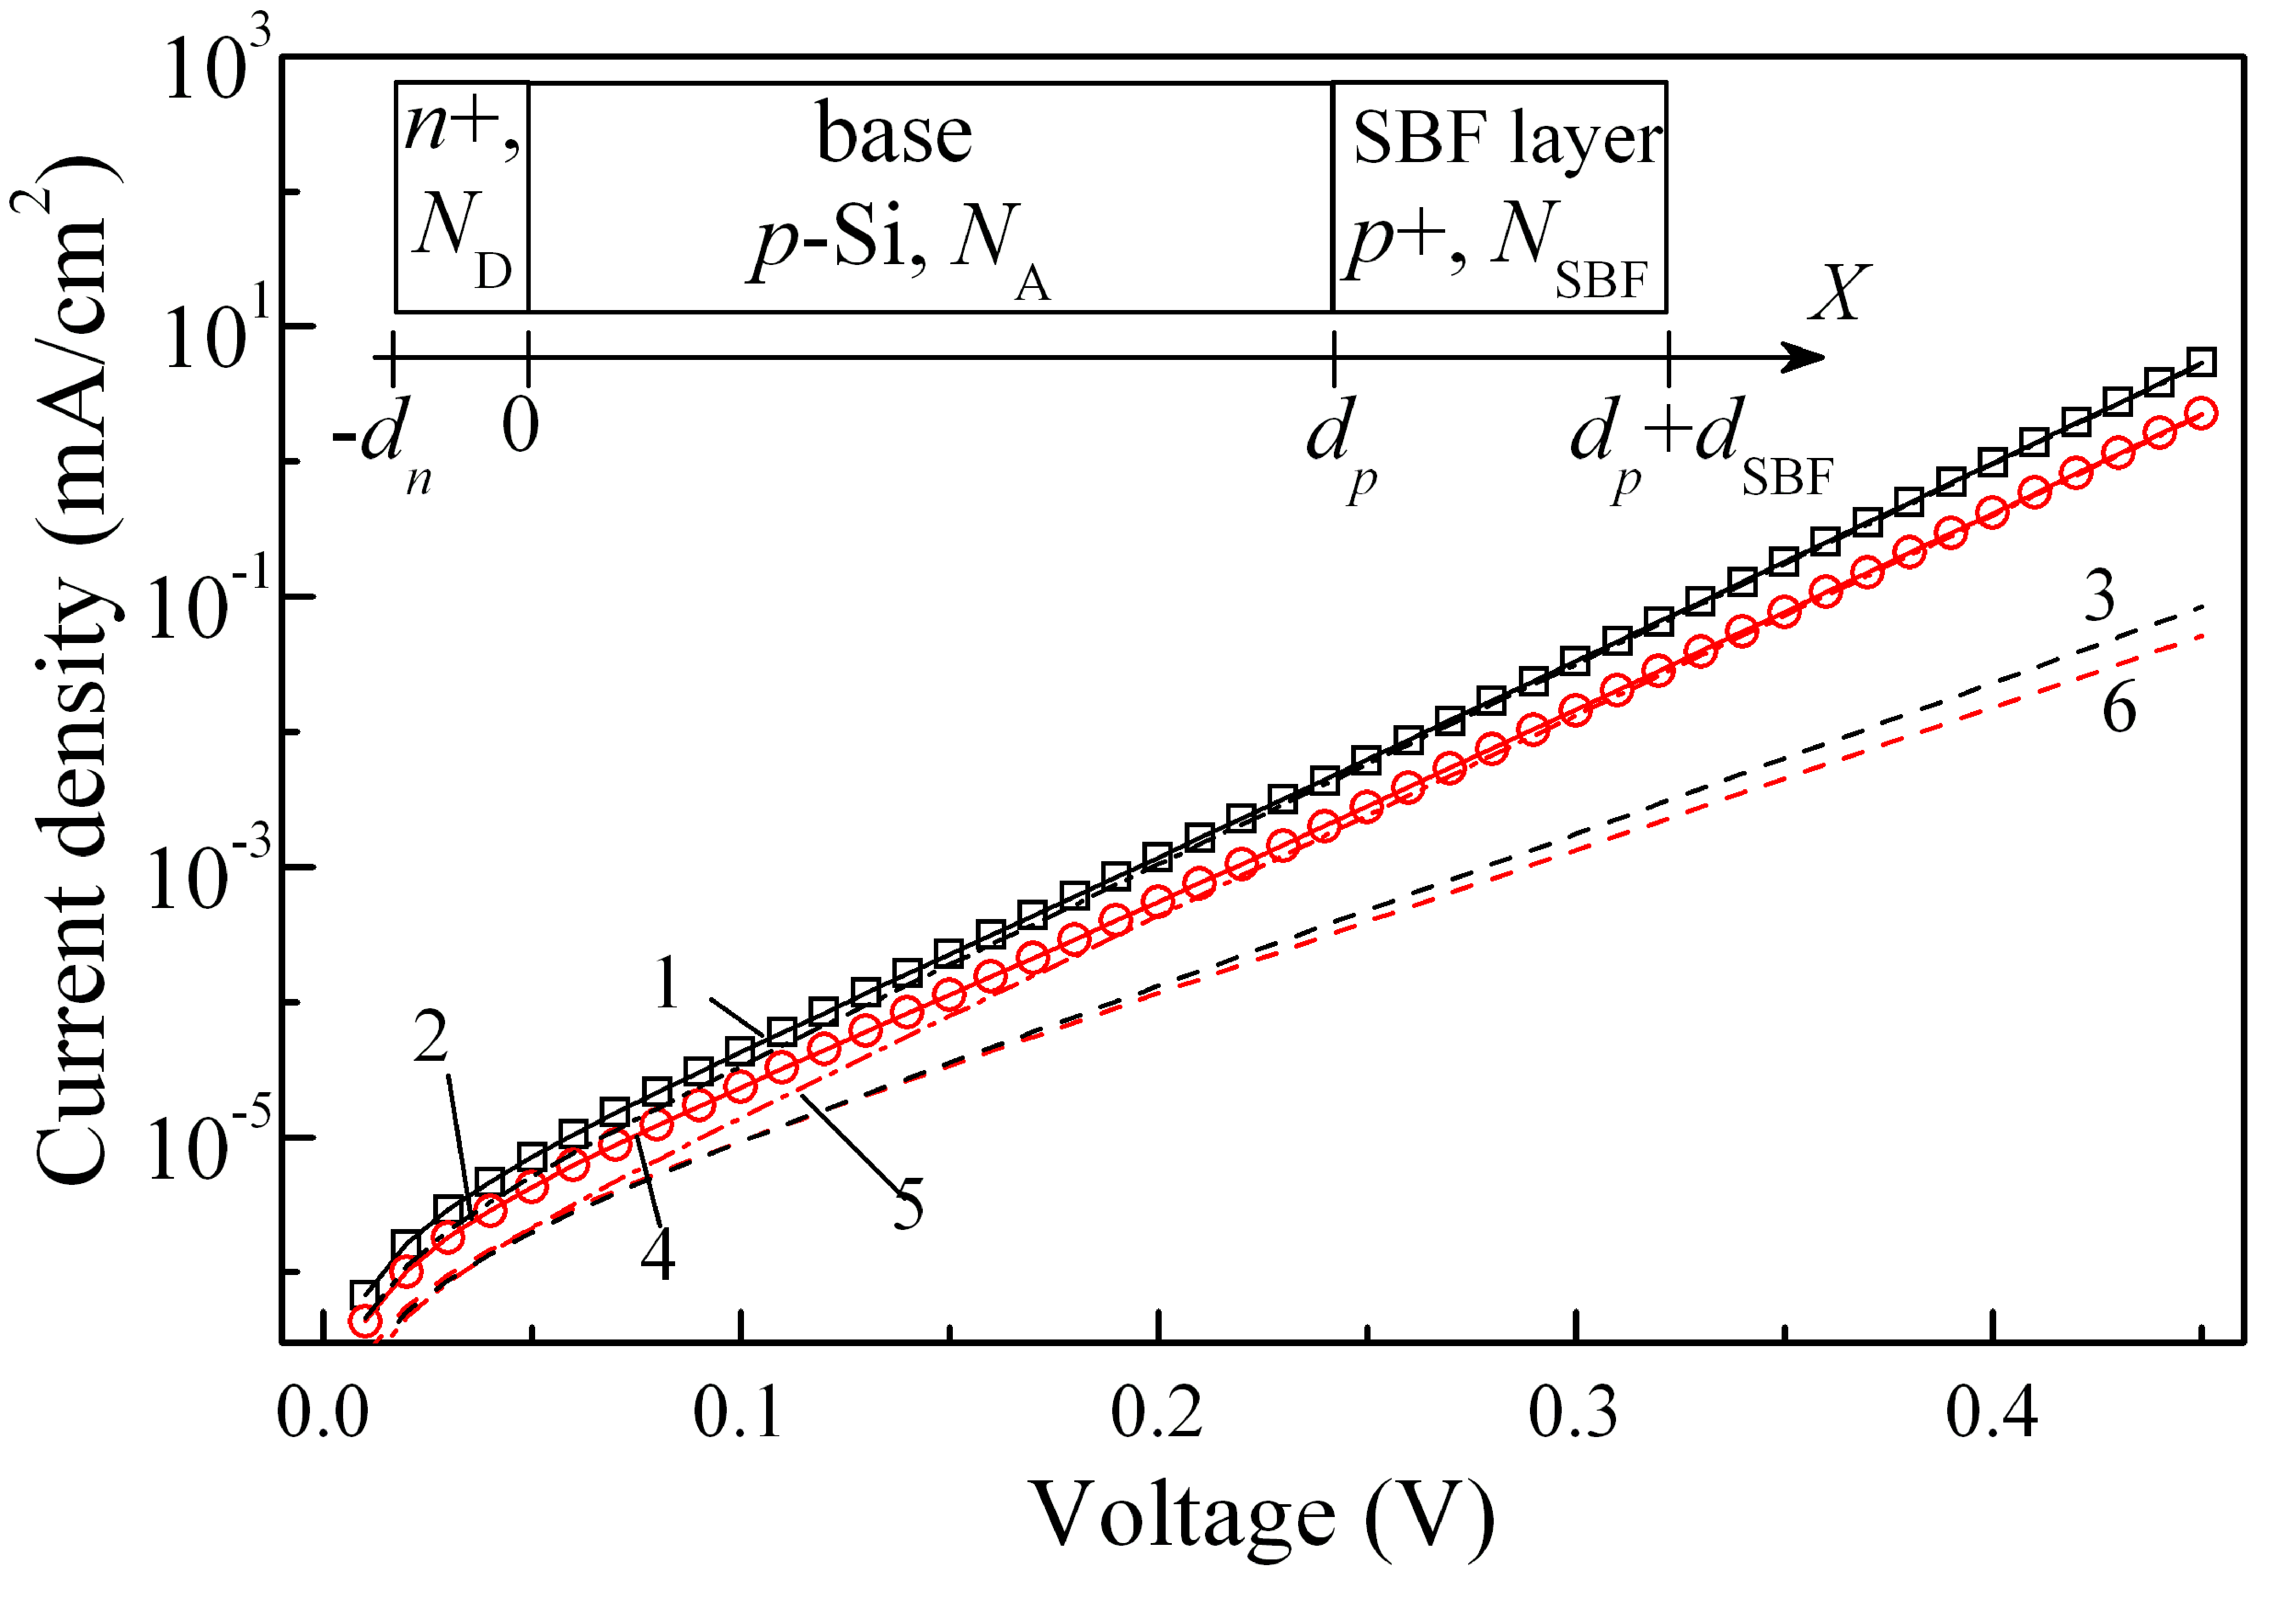
\includegraphics[width=7.5cm]{FigIV}
\caption{.
}
\label{FigIV}
\end{figure}


\begin{figure}
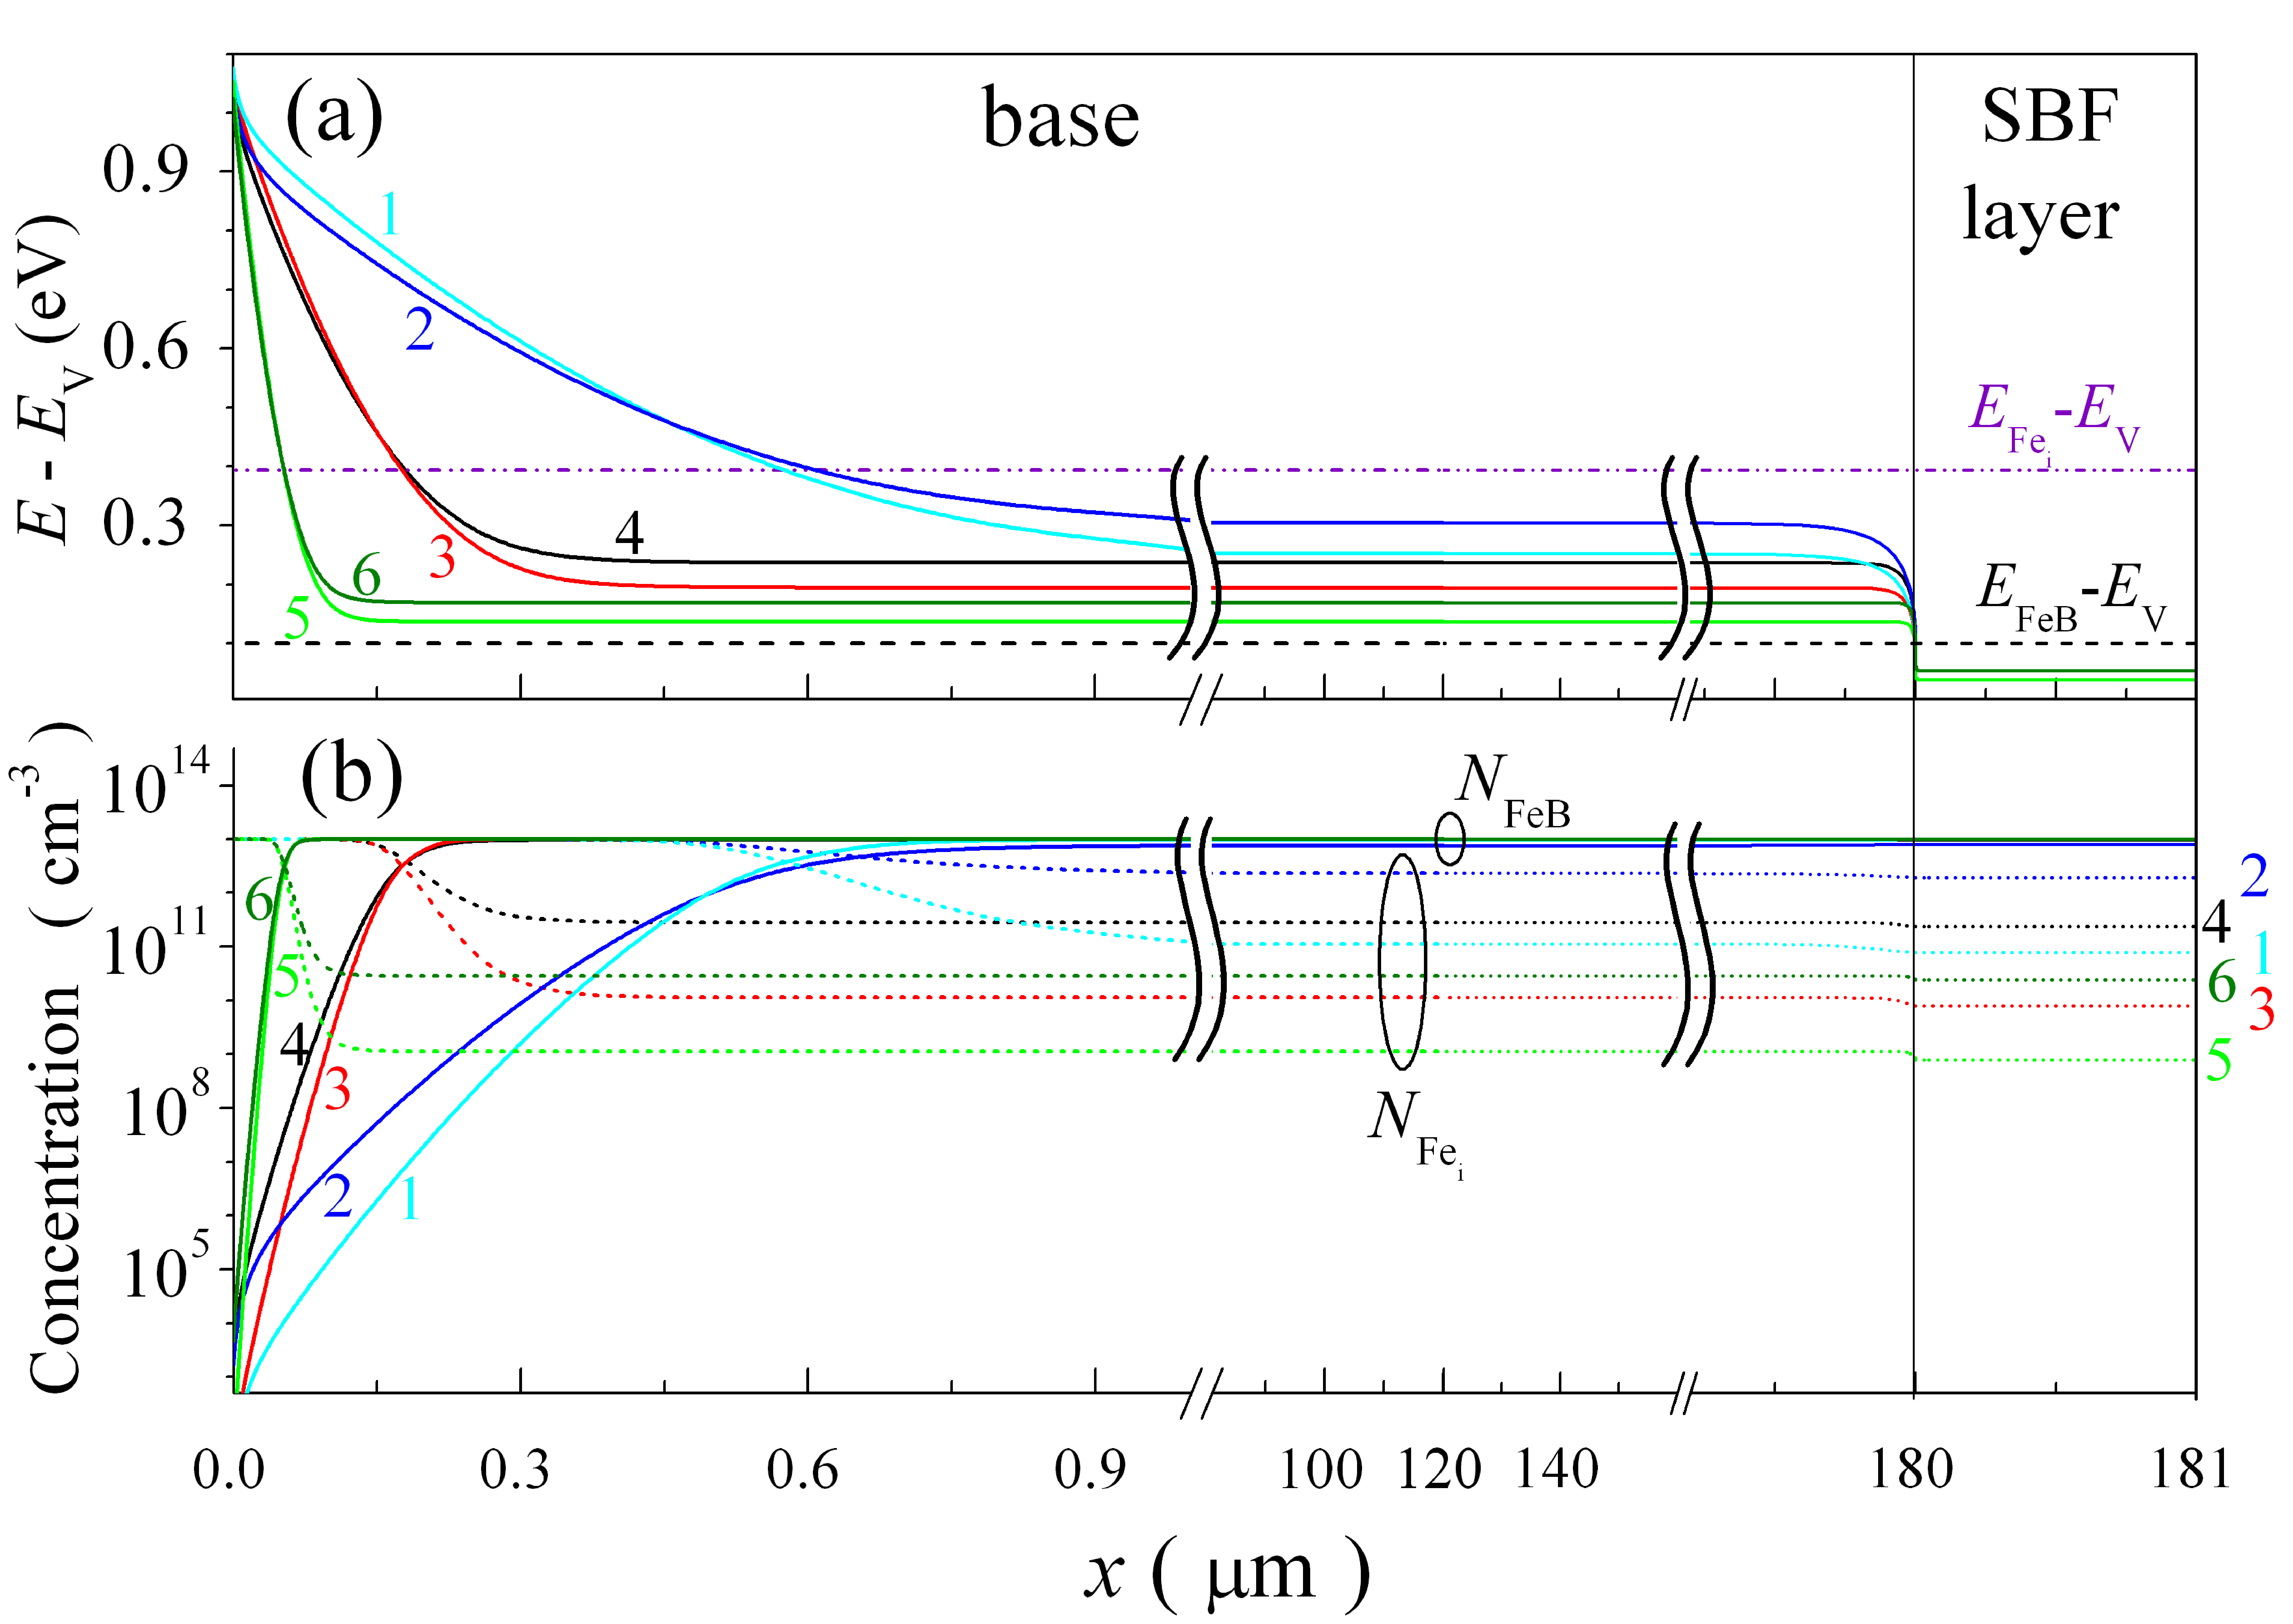
\includegraphics[width=15cm]{FigEfAll}
\caption{.
}
\label{FigEf}
\end{figure}

\begin{figure}
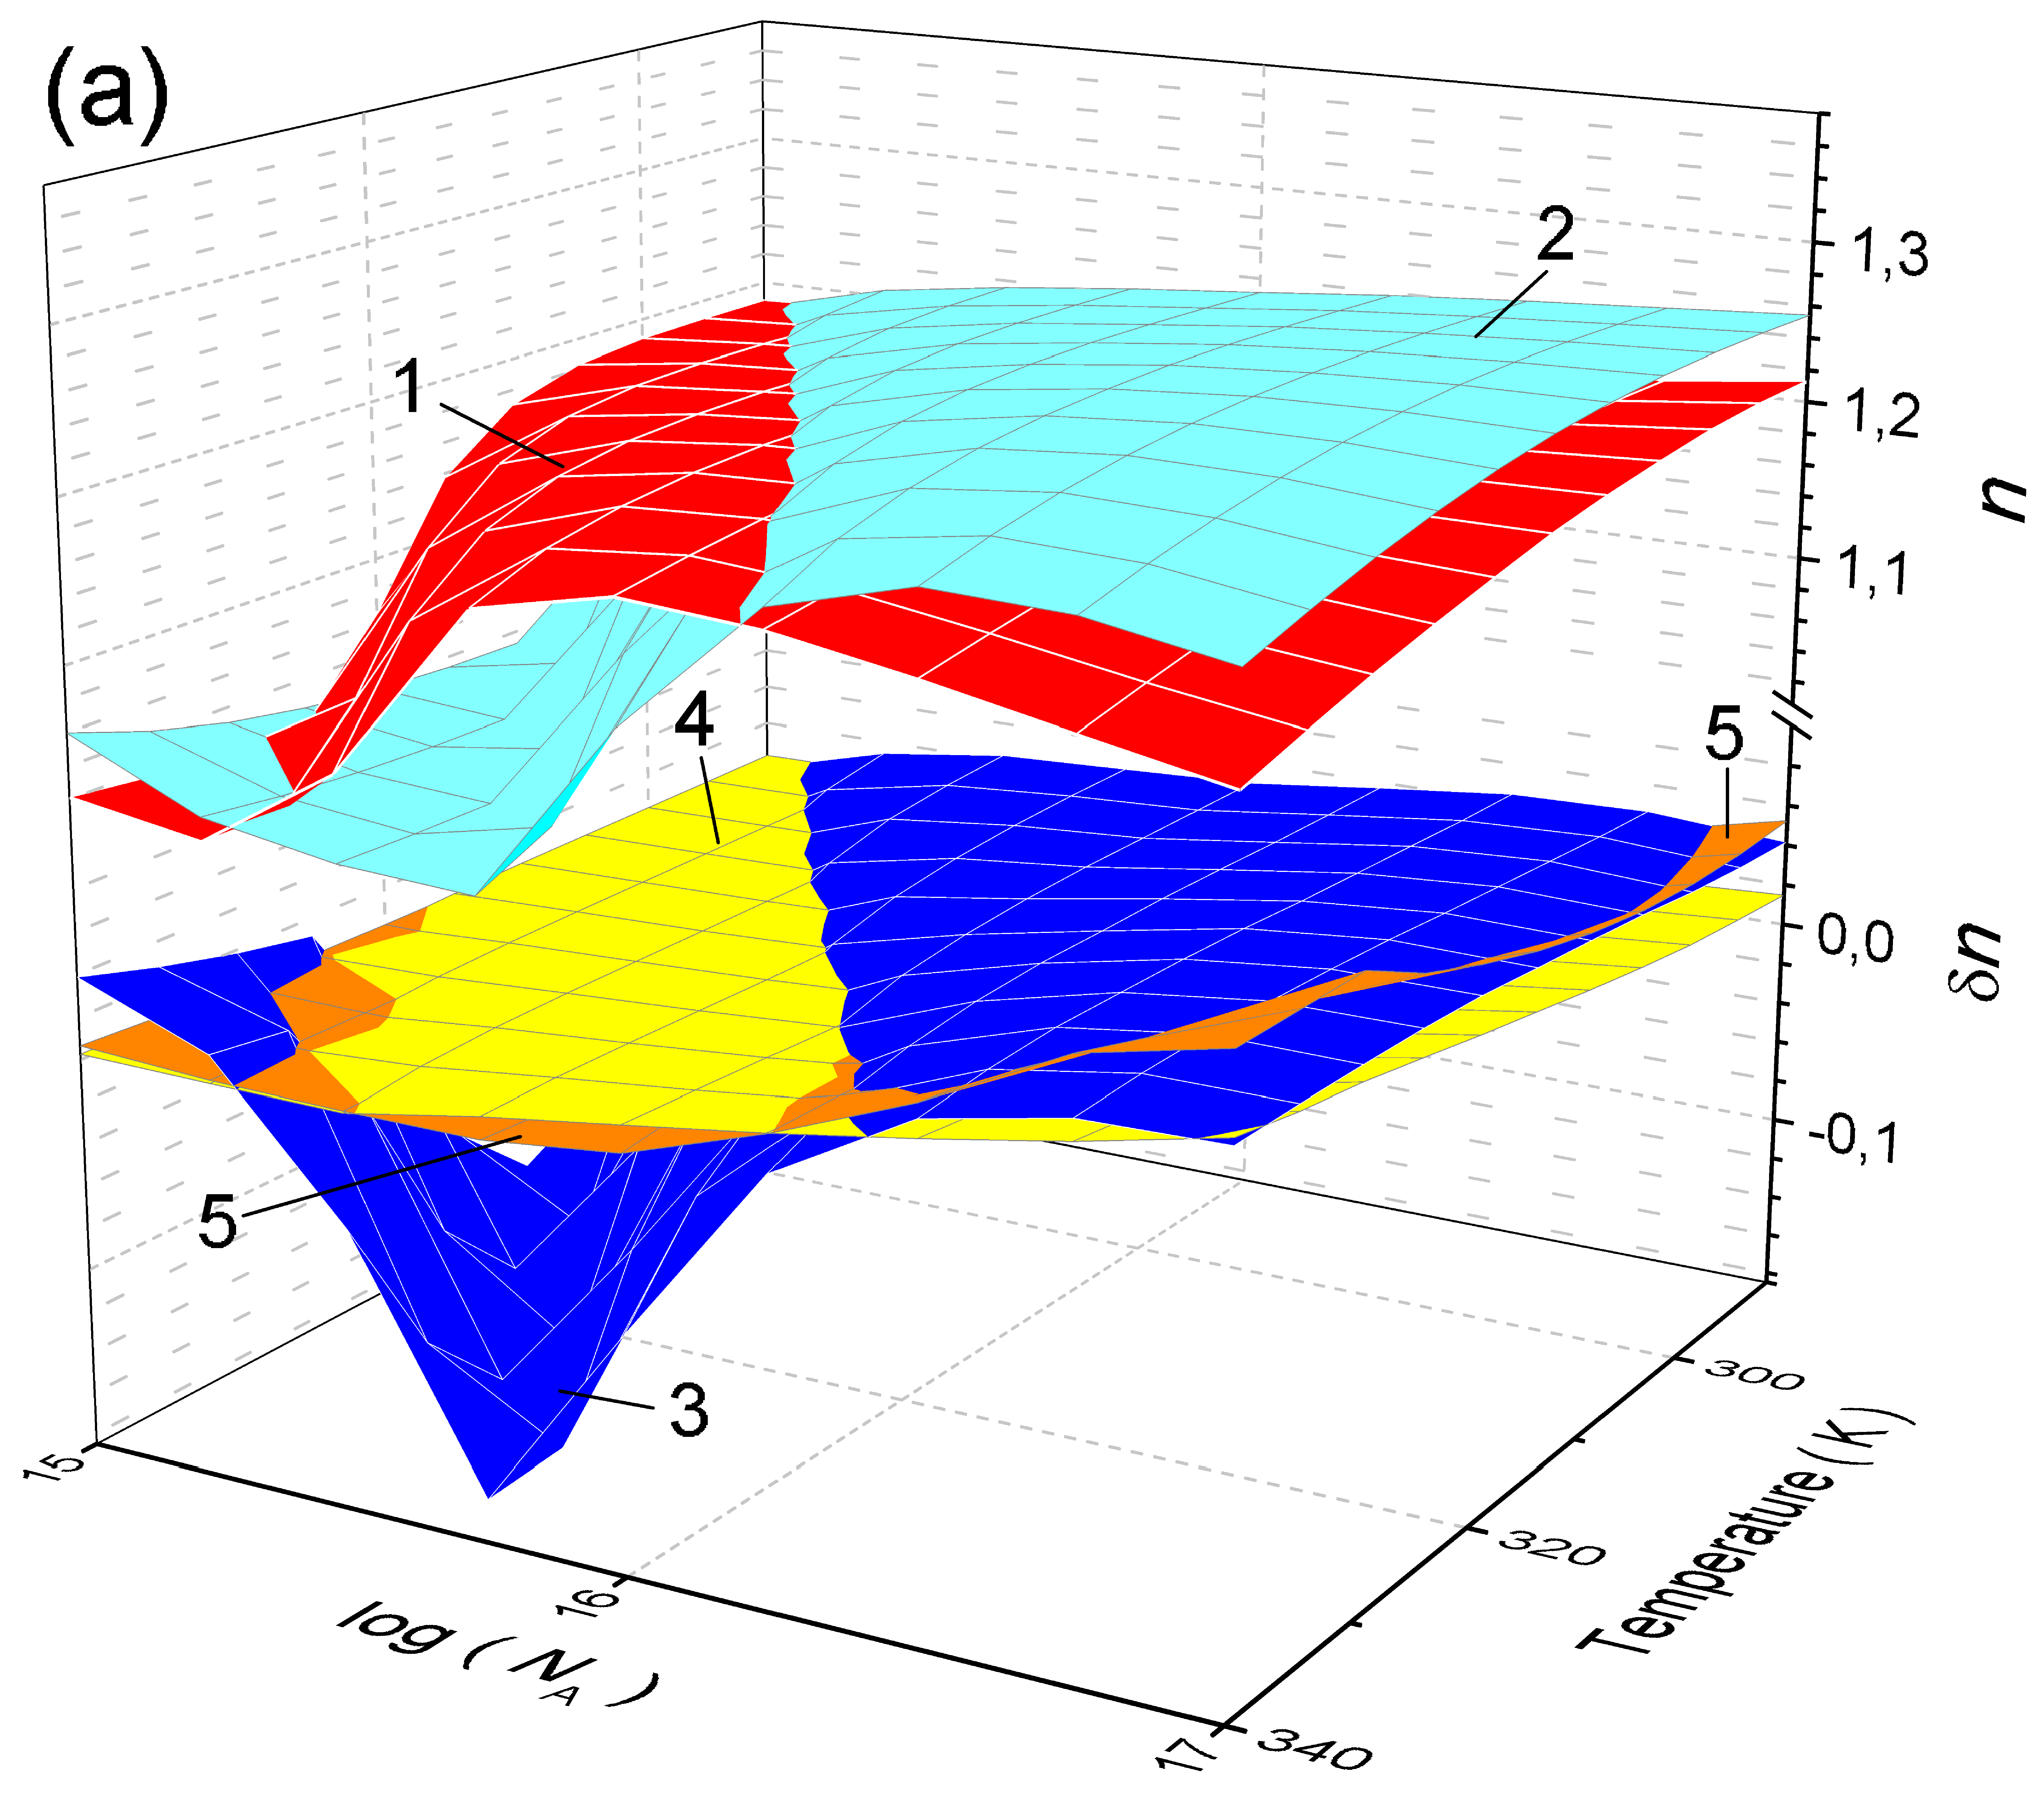
\includegraphics[width=7.5cm]{FigFe100d24} \hfill
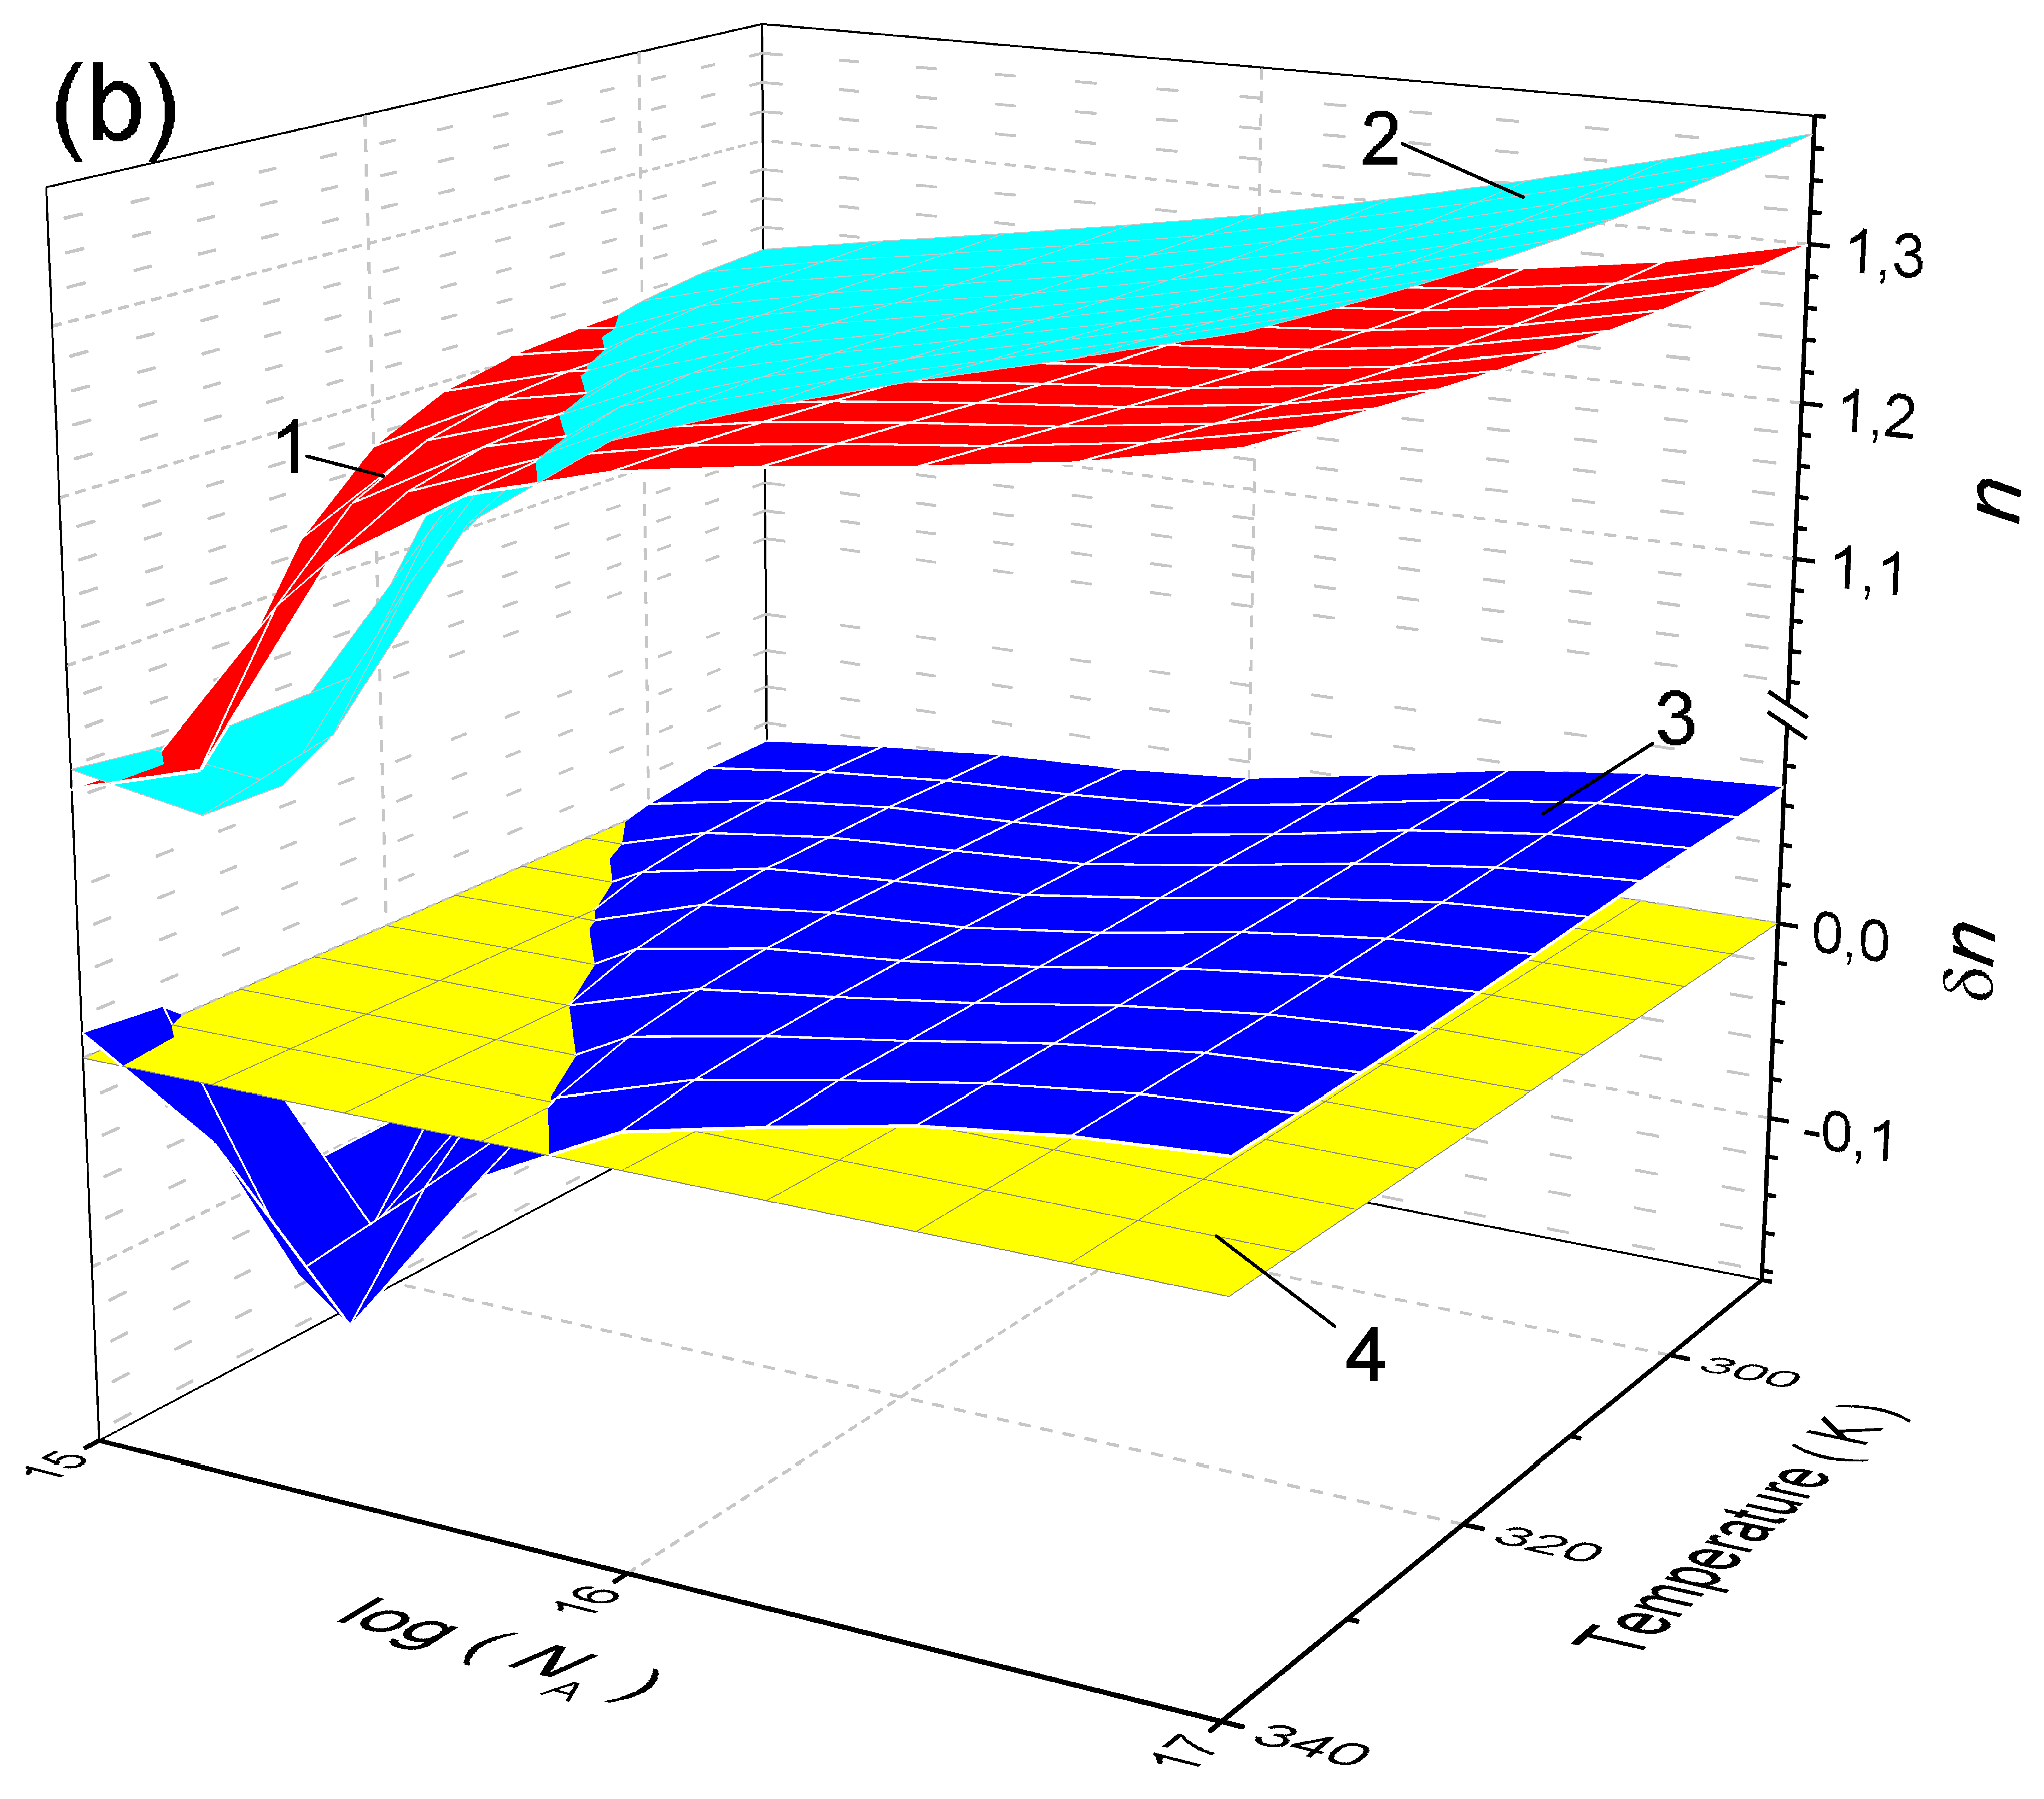
\includegraphics[width=7.5cm]{FigFe103d24}
\caption{.
}
\label{FigTNa}
\end{figure}

\begin{figure}
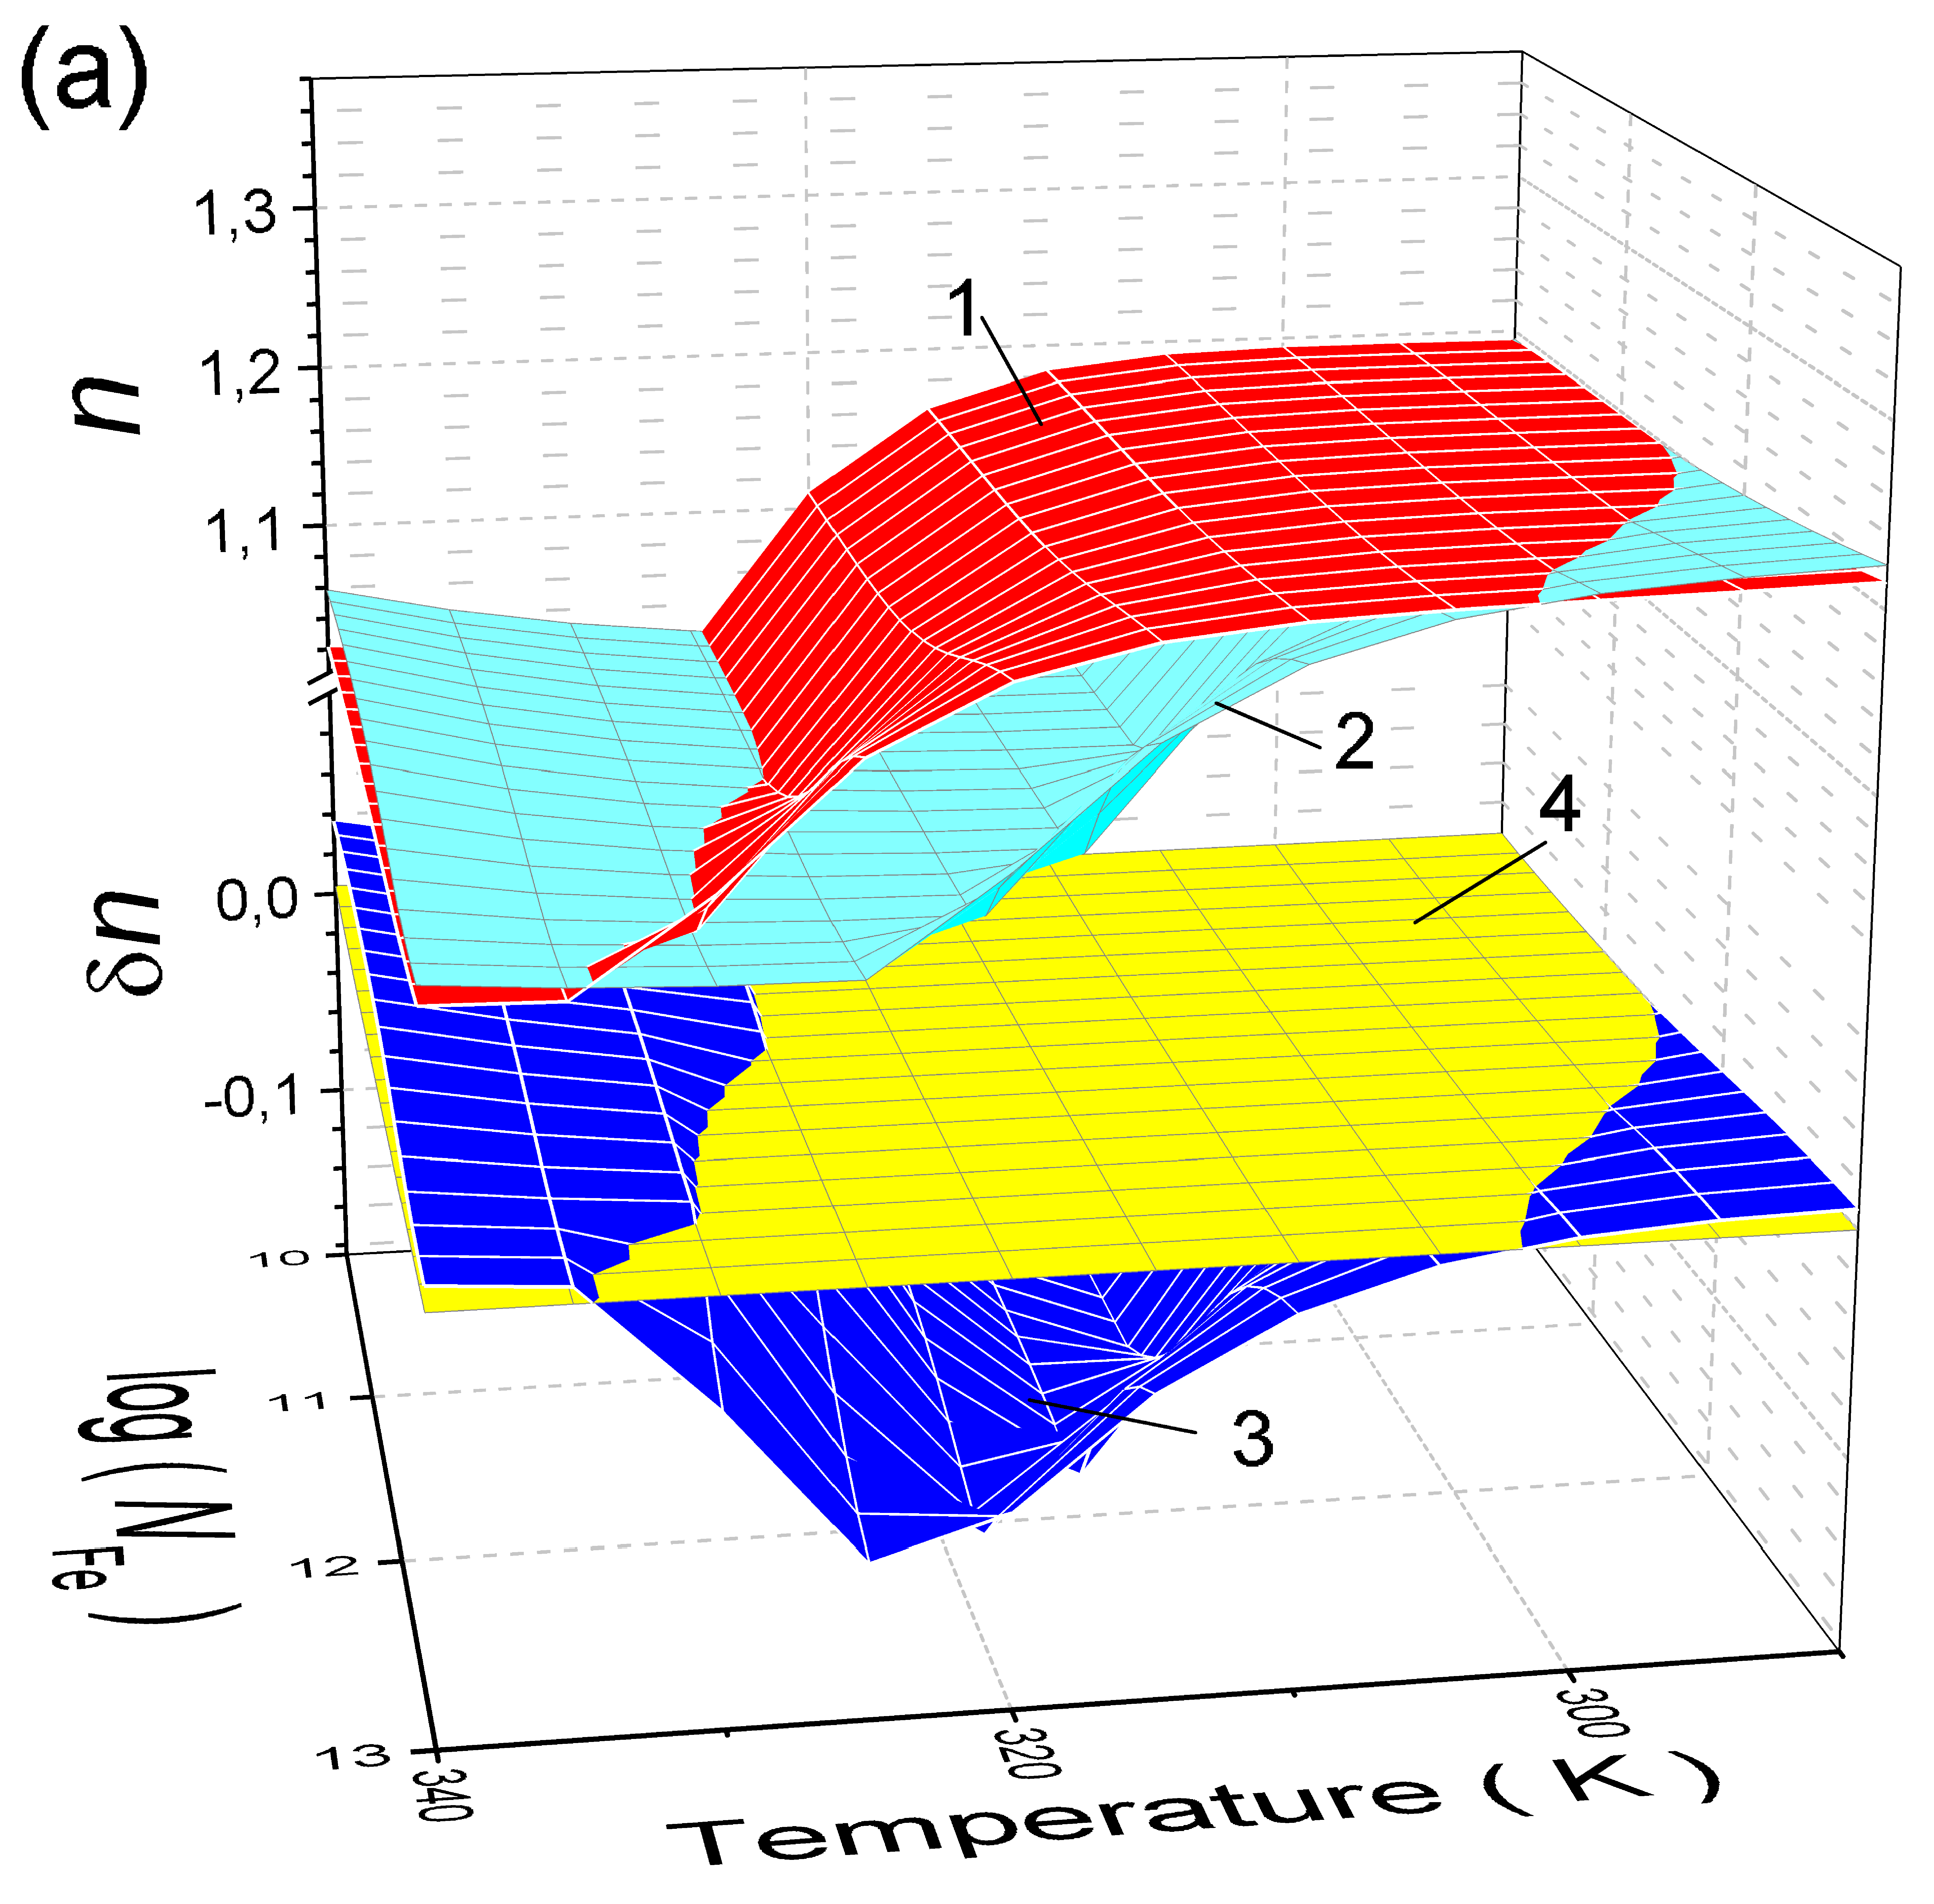
\includegraphics[width=4.9cm]{FigB105d15} \hfill
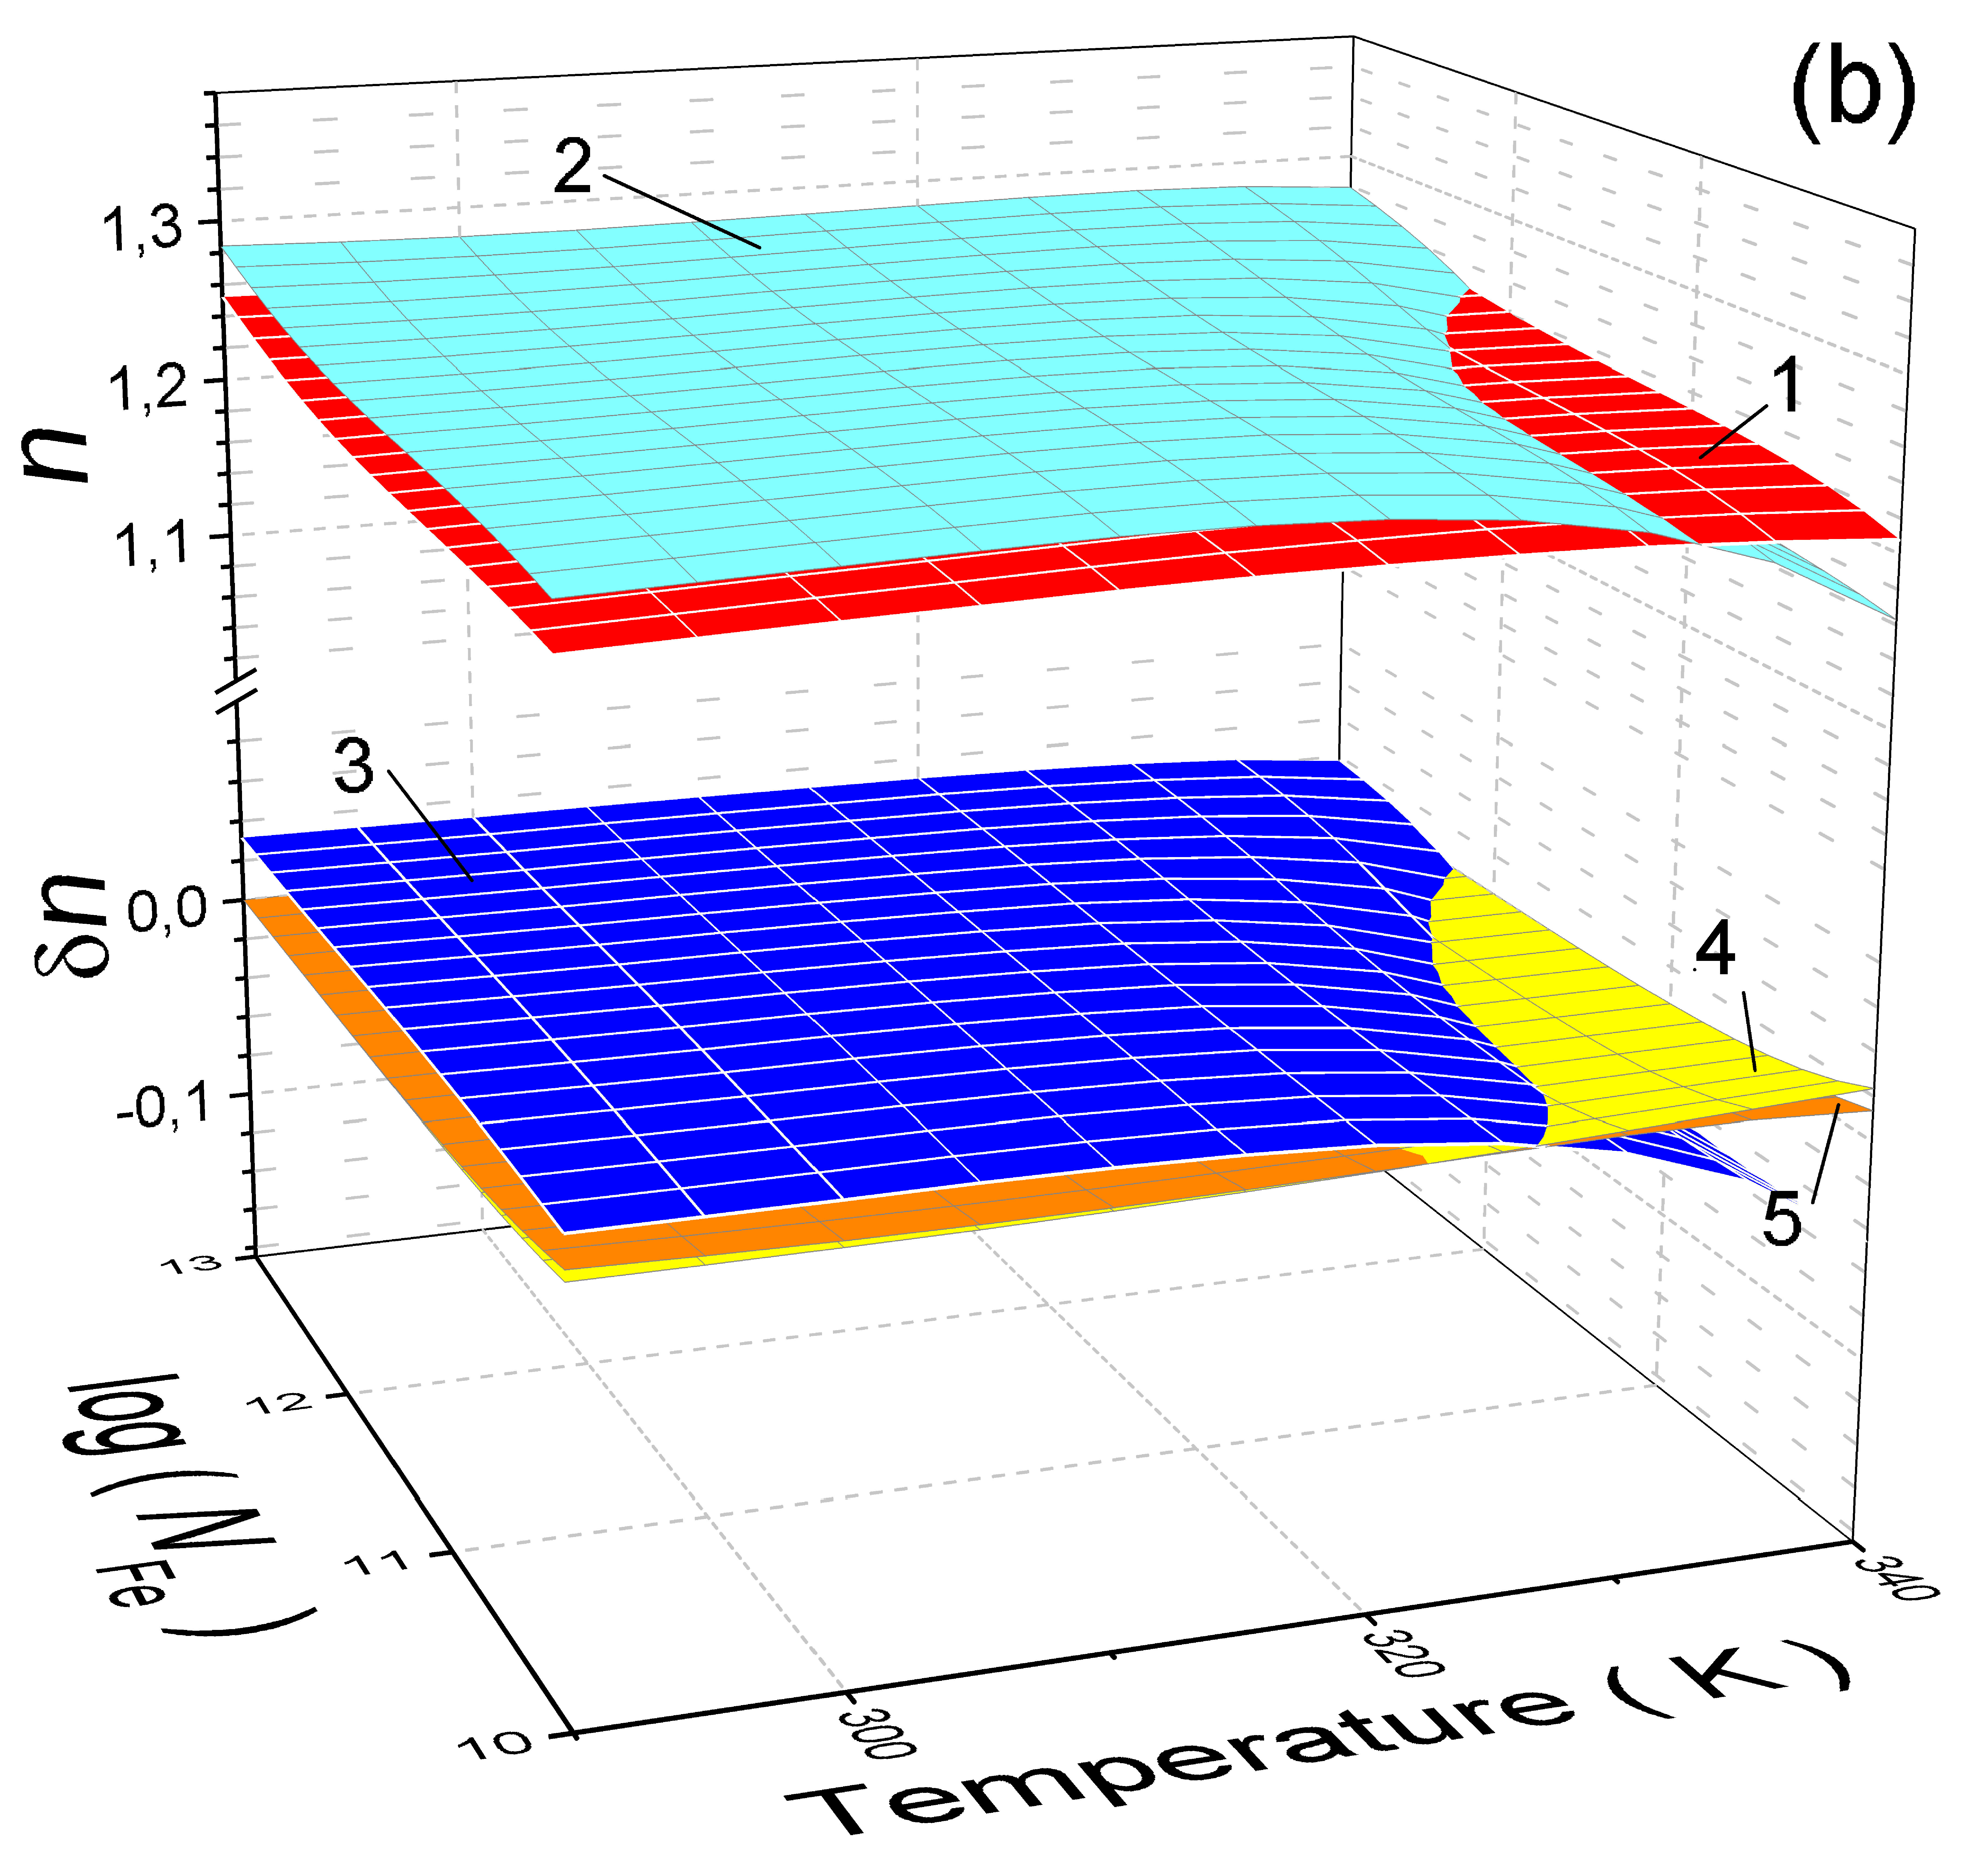
\includegraphics[width=4.9cm]{FigB106d15} \hfill
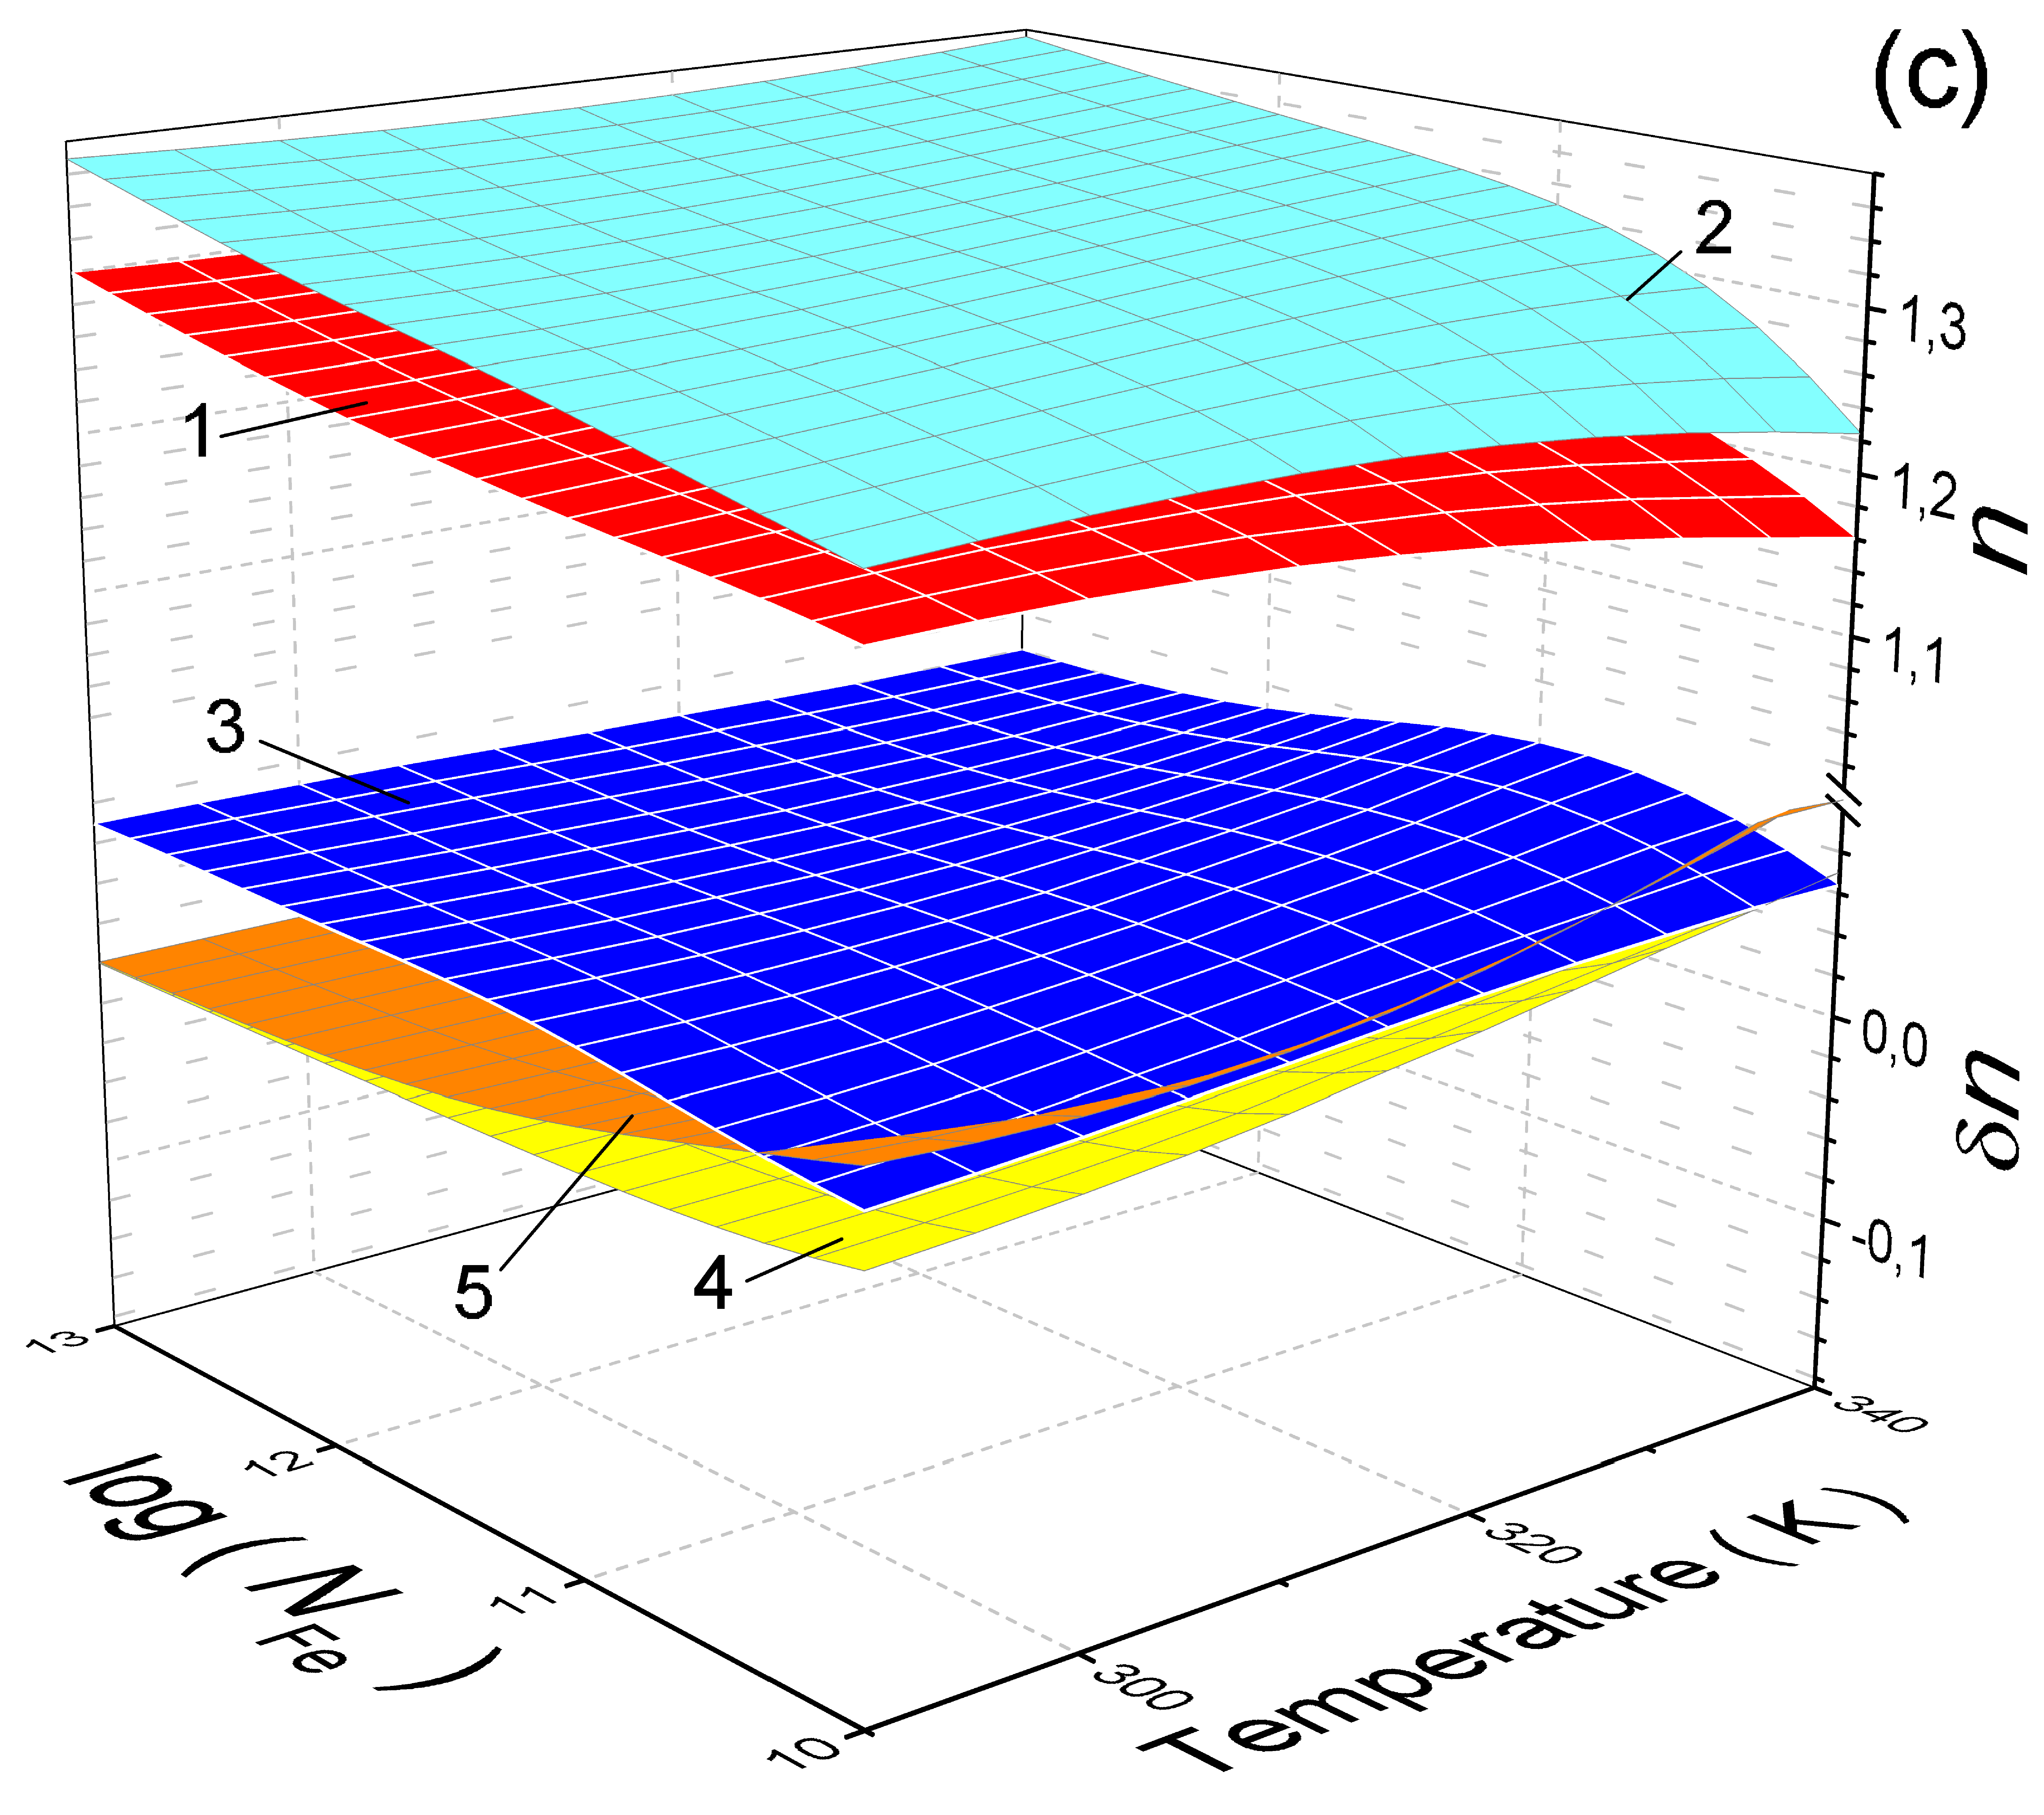
\includegraphics[width=4.9cm]{FigB107d15}
\caption{.
}
\label{FigTNfe}
\end{figure}

\begin{figure}
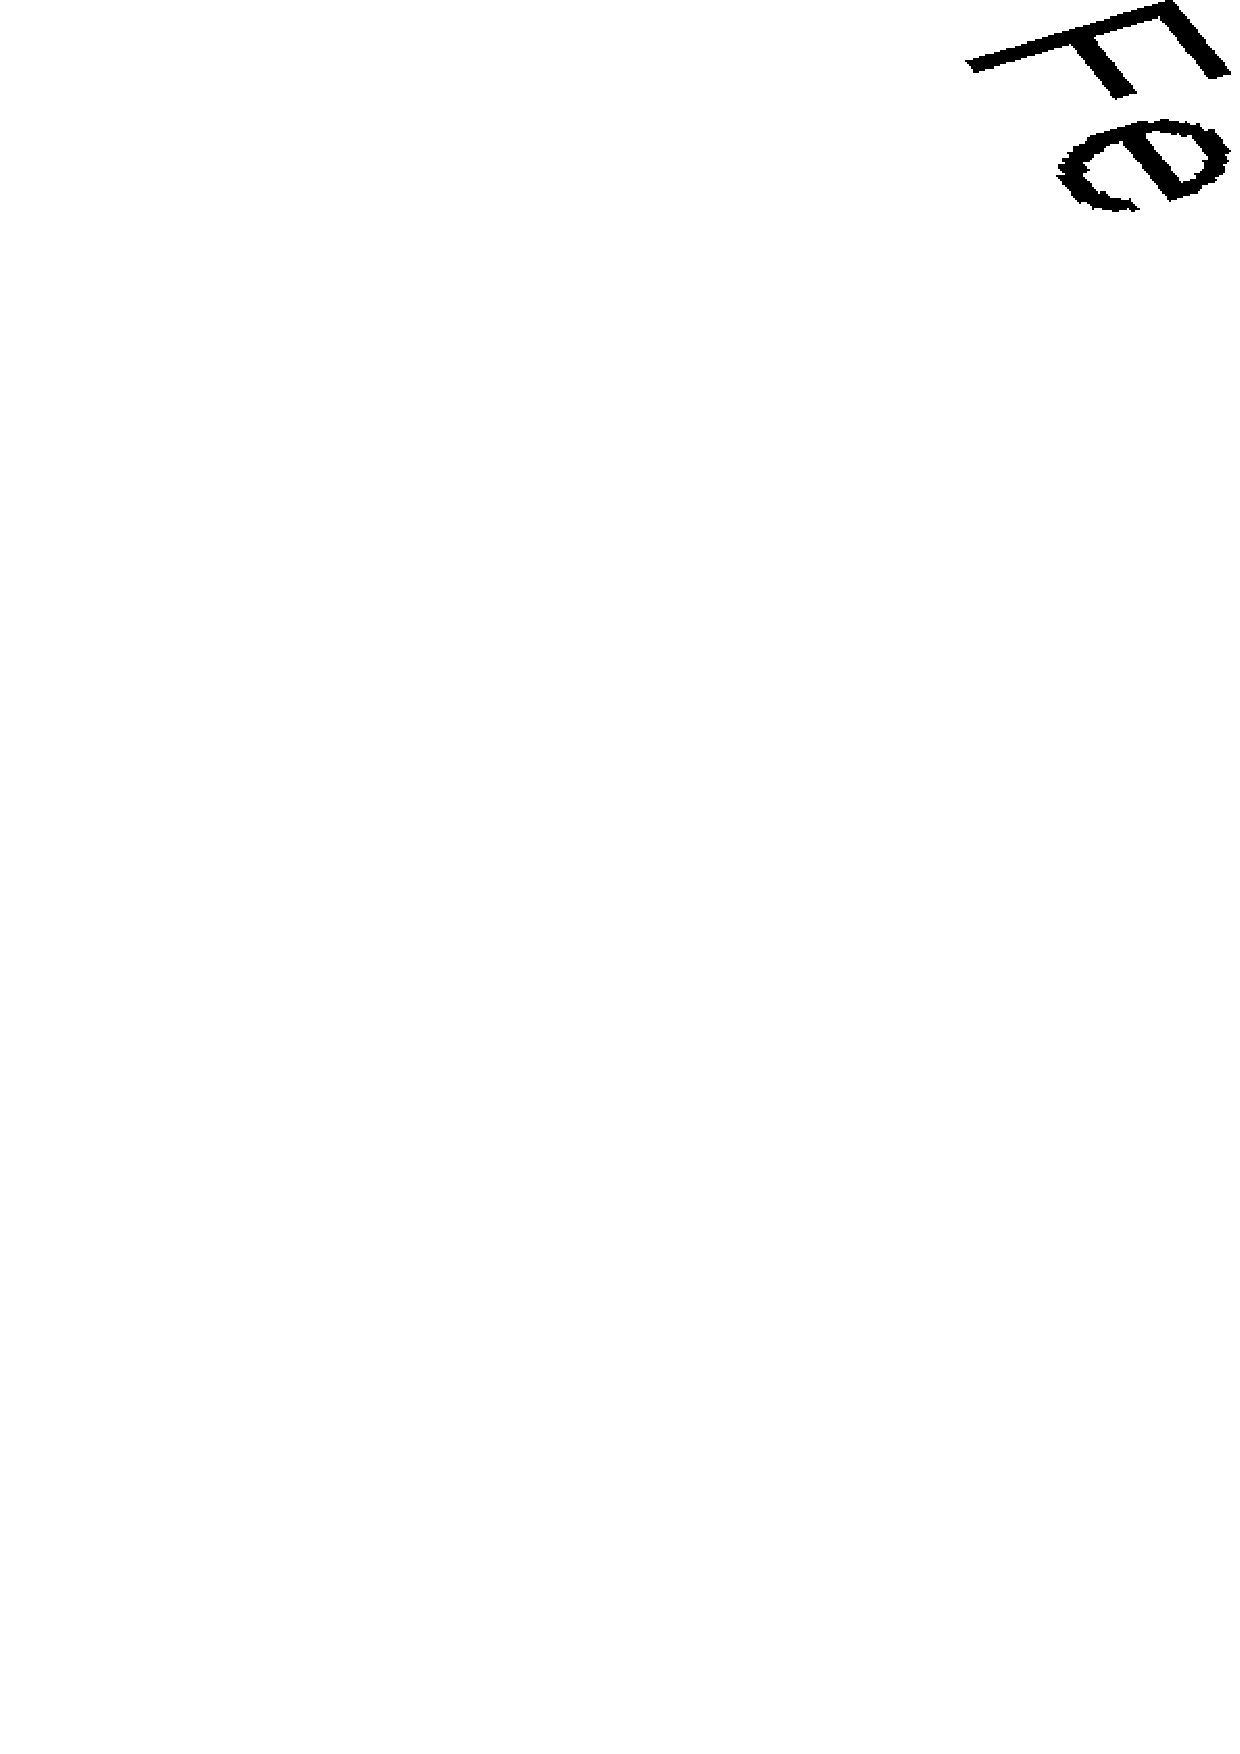
\includegraphics[width=7.5cm]{FigT290d18} \hfill
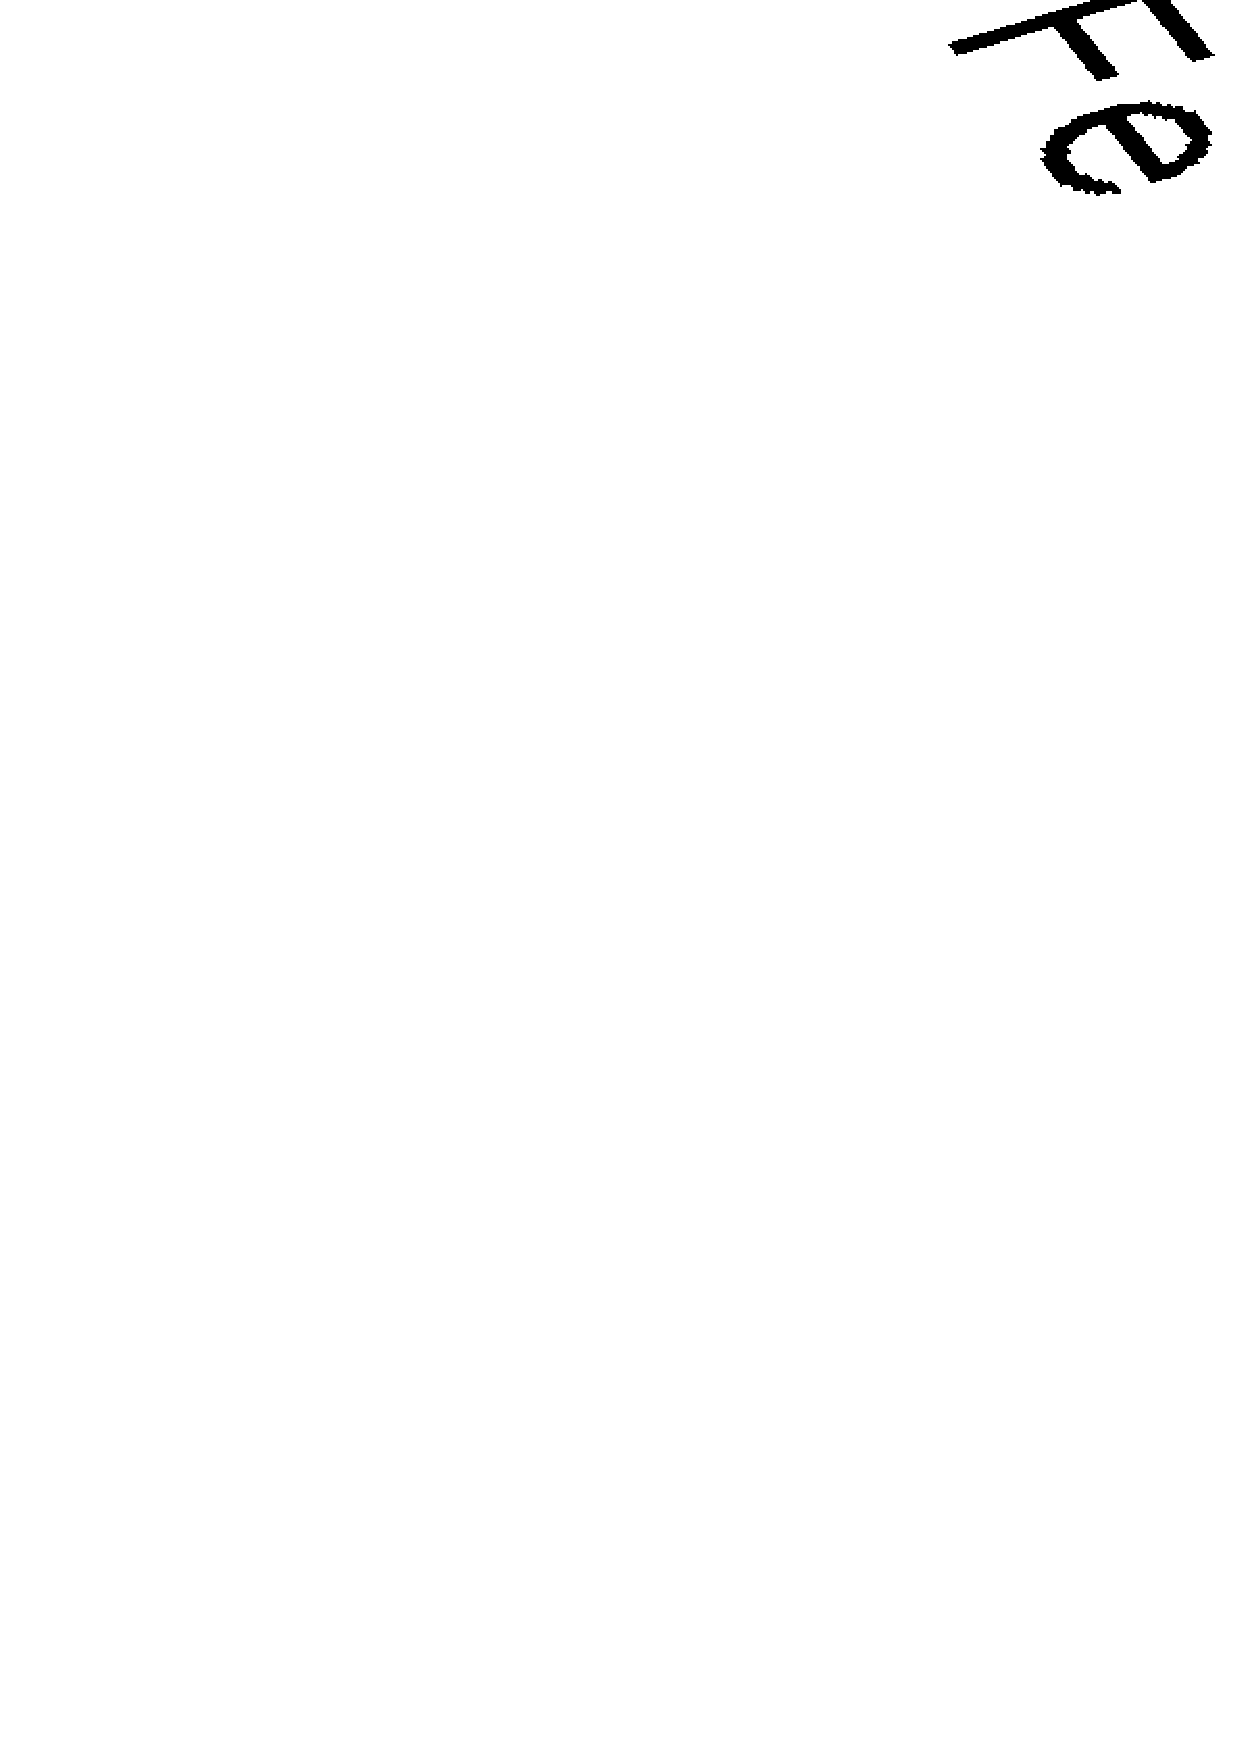
\includegraphics[width=7.5cm]{FigT340d18}
\caption{.
}
\label{FigNaNfe}
\end{figure}

\begin{figure}
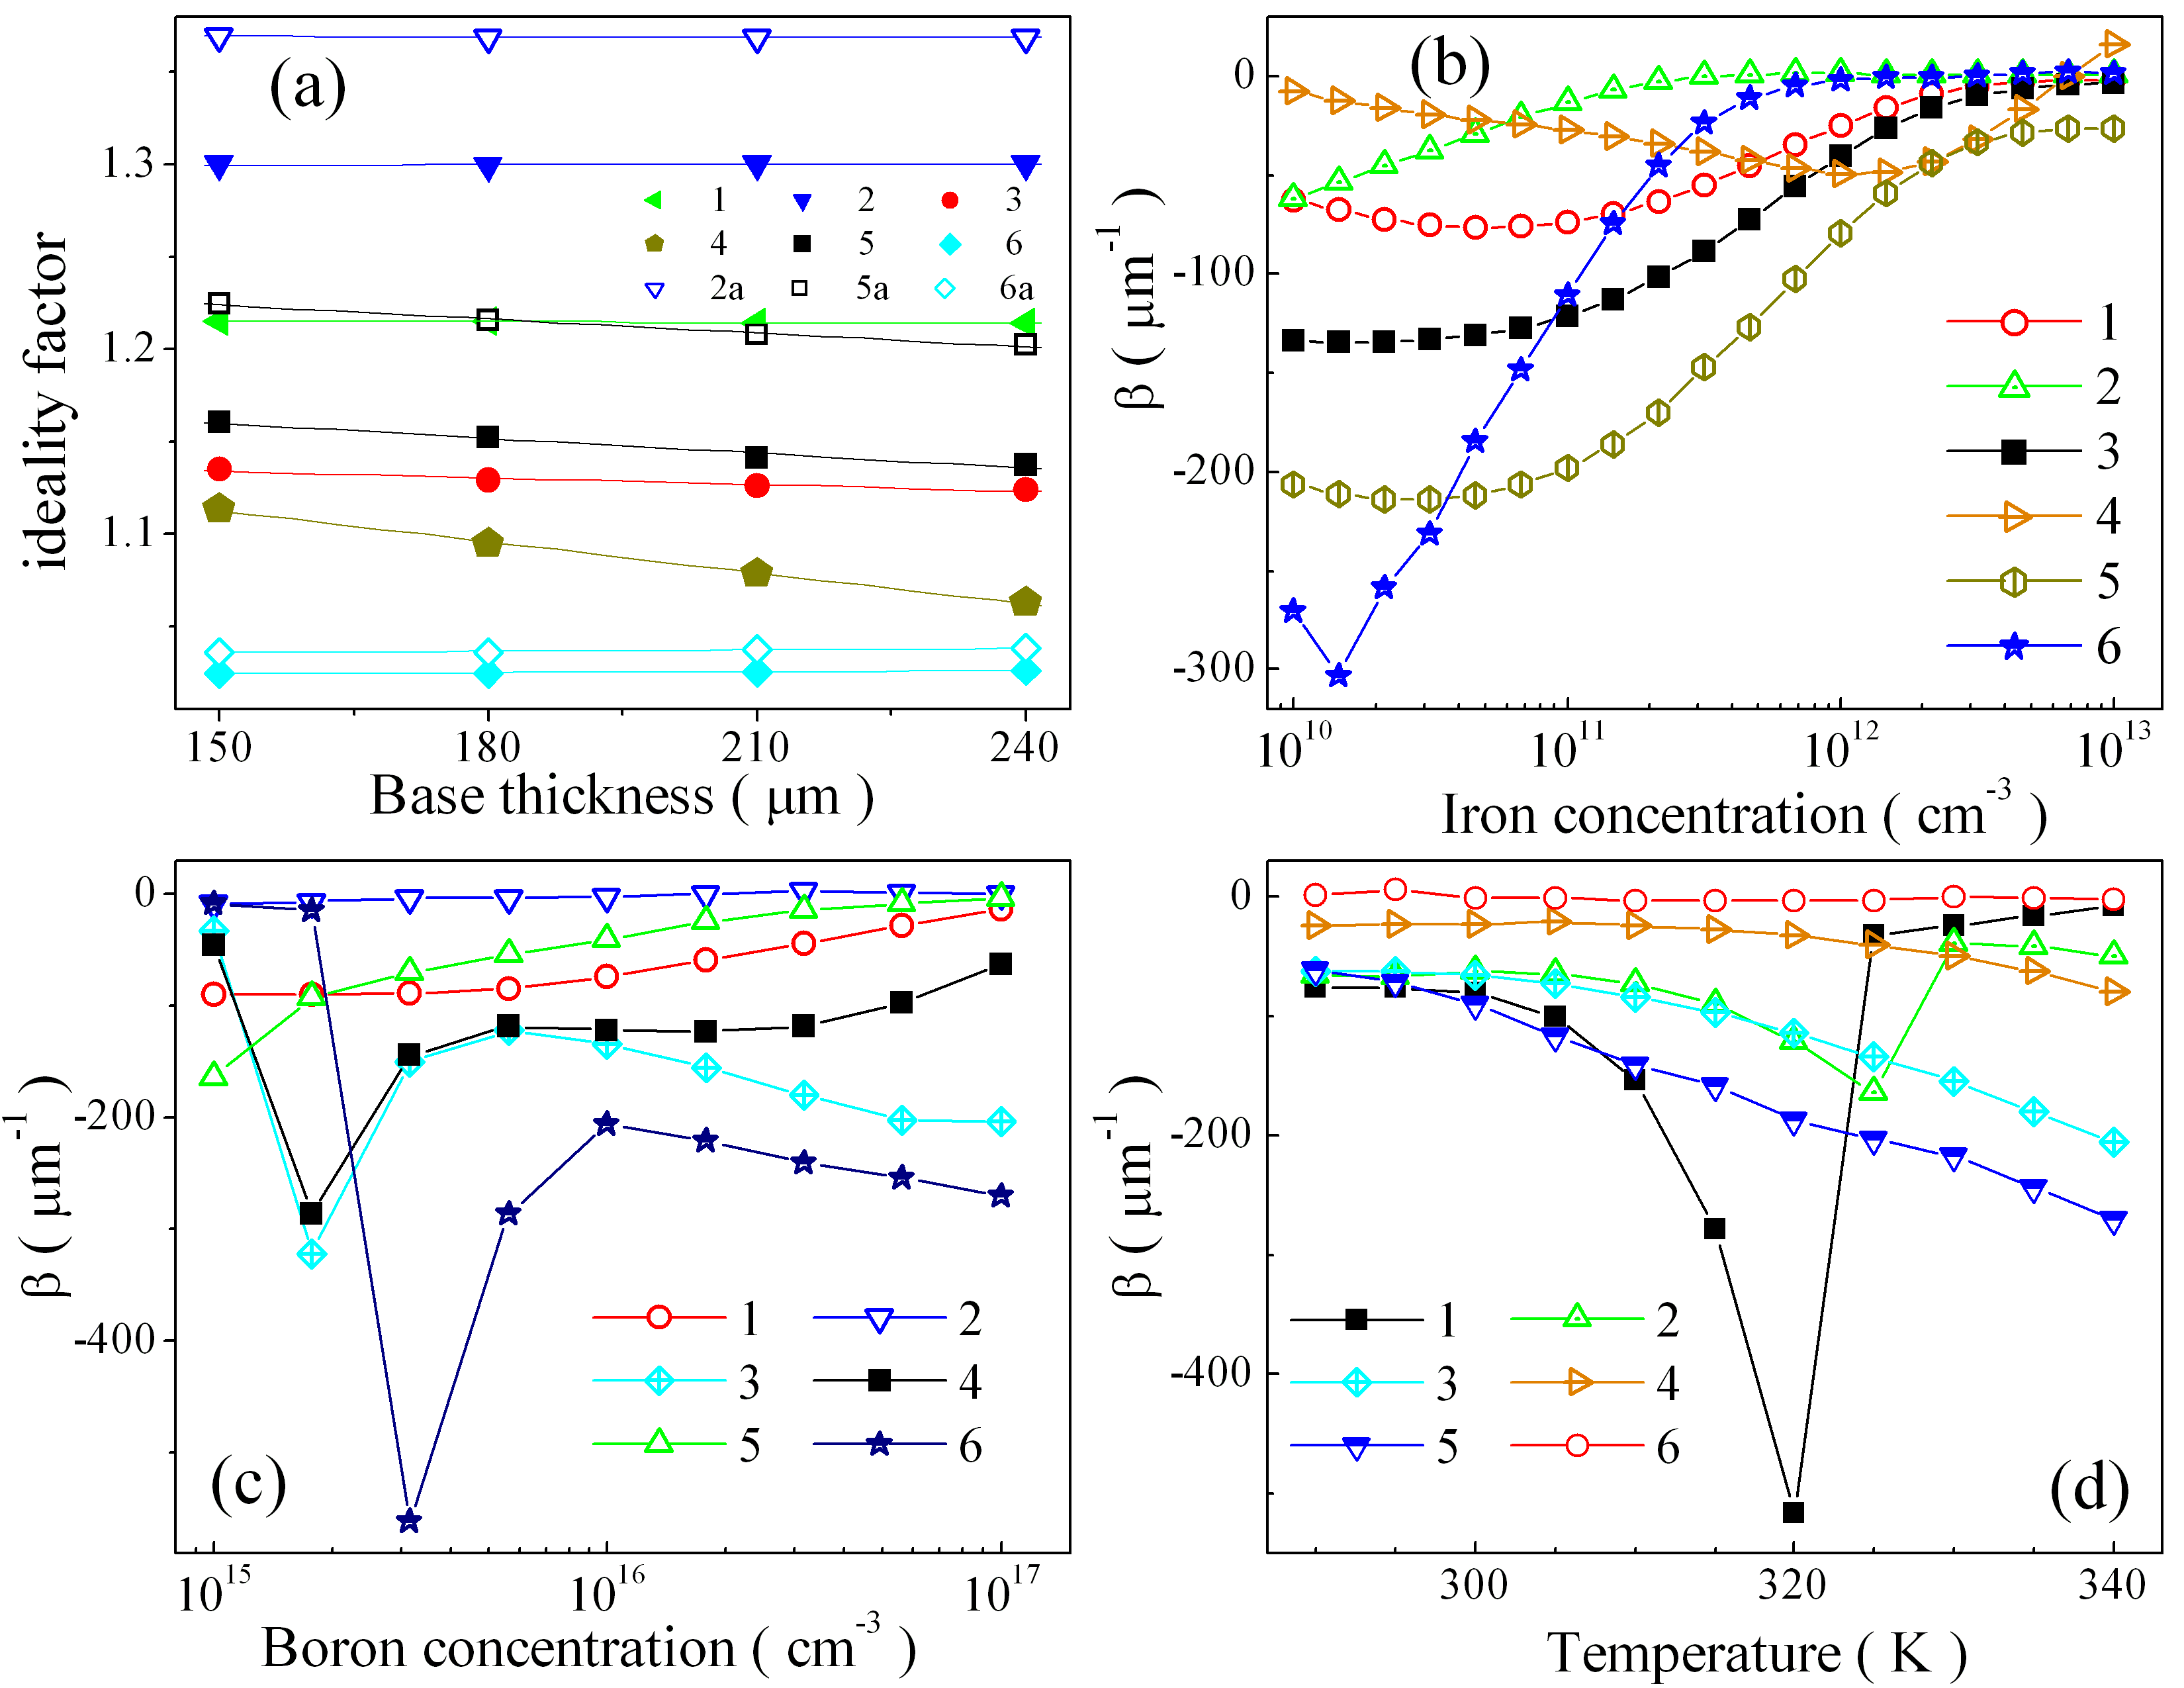
\includegraphics[width=15cm]{FigTotal}
\caption{.
}
\label{FigTotal}
\end{figure}


\begin{figure}
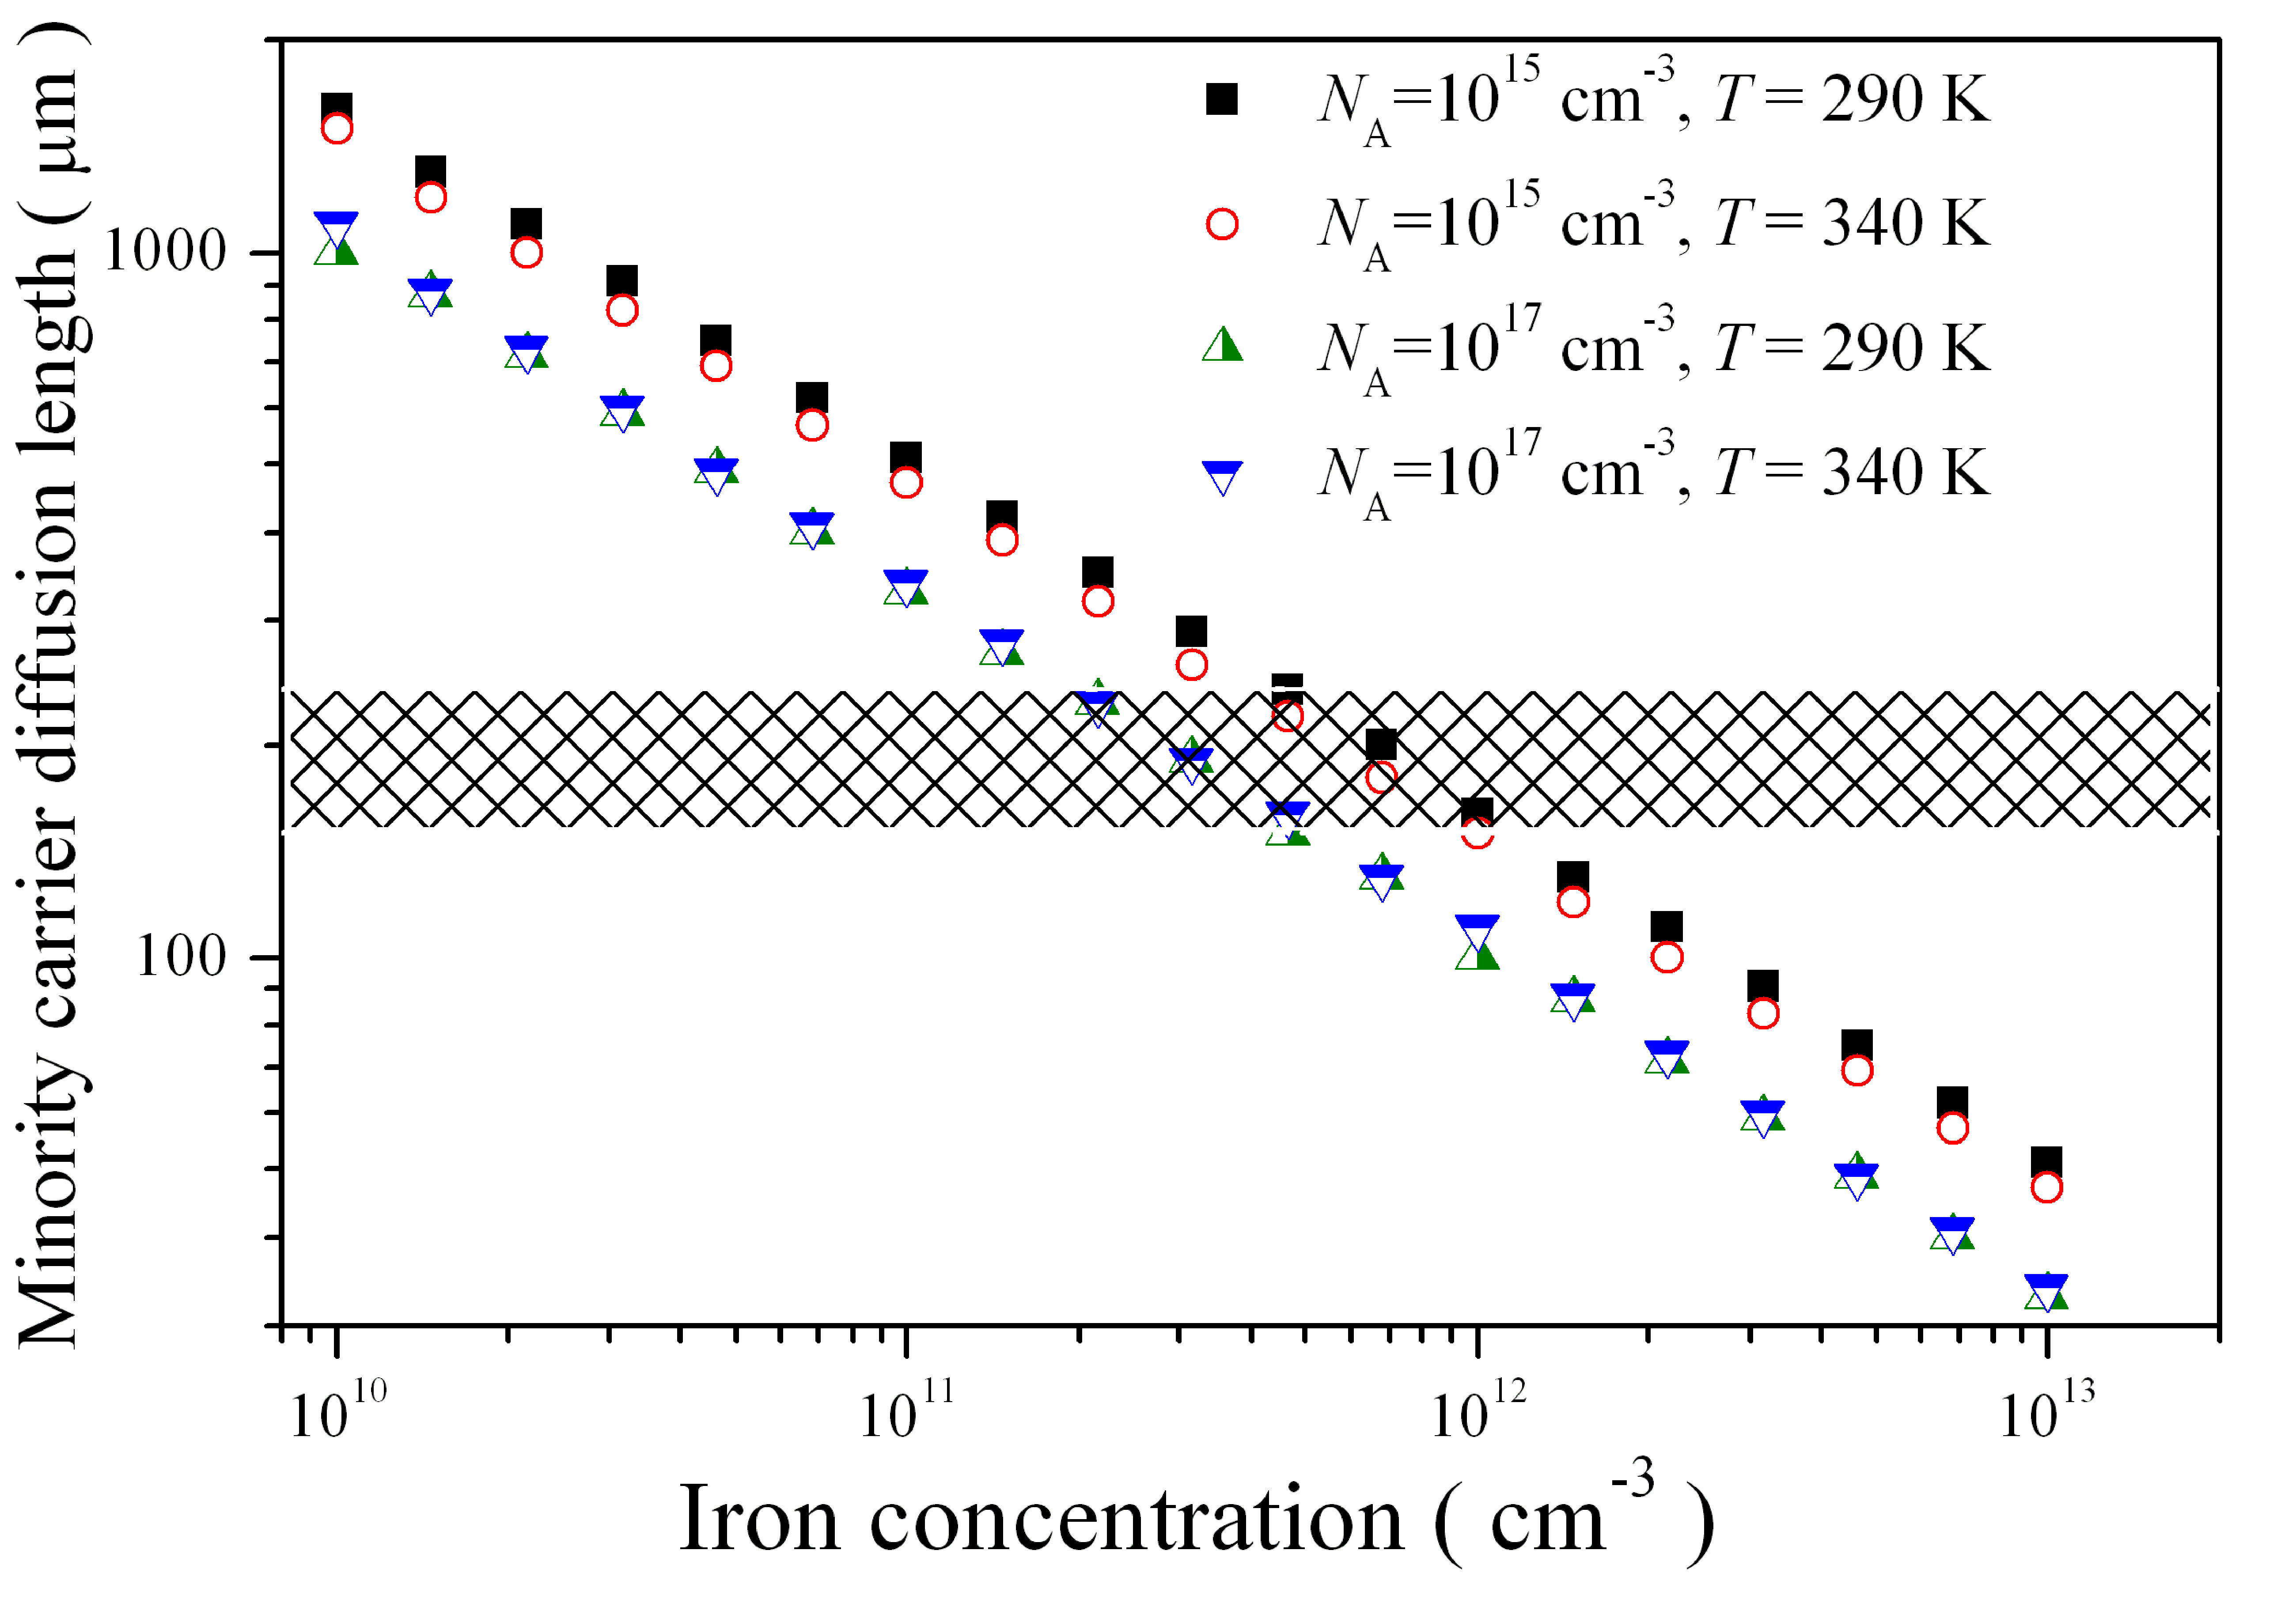
\includegraphics[width=7.5cm]{FigLn}
\caption{.
}
\label{FigLn}
\end{figure}

\begin{figure}
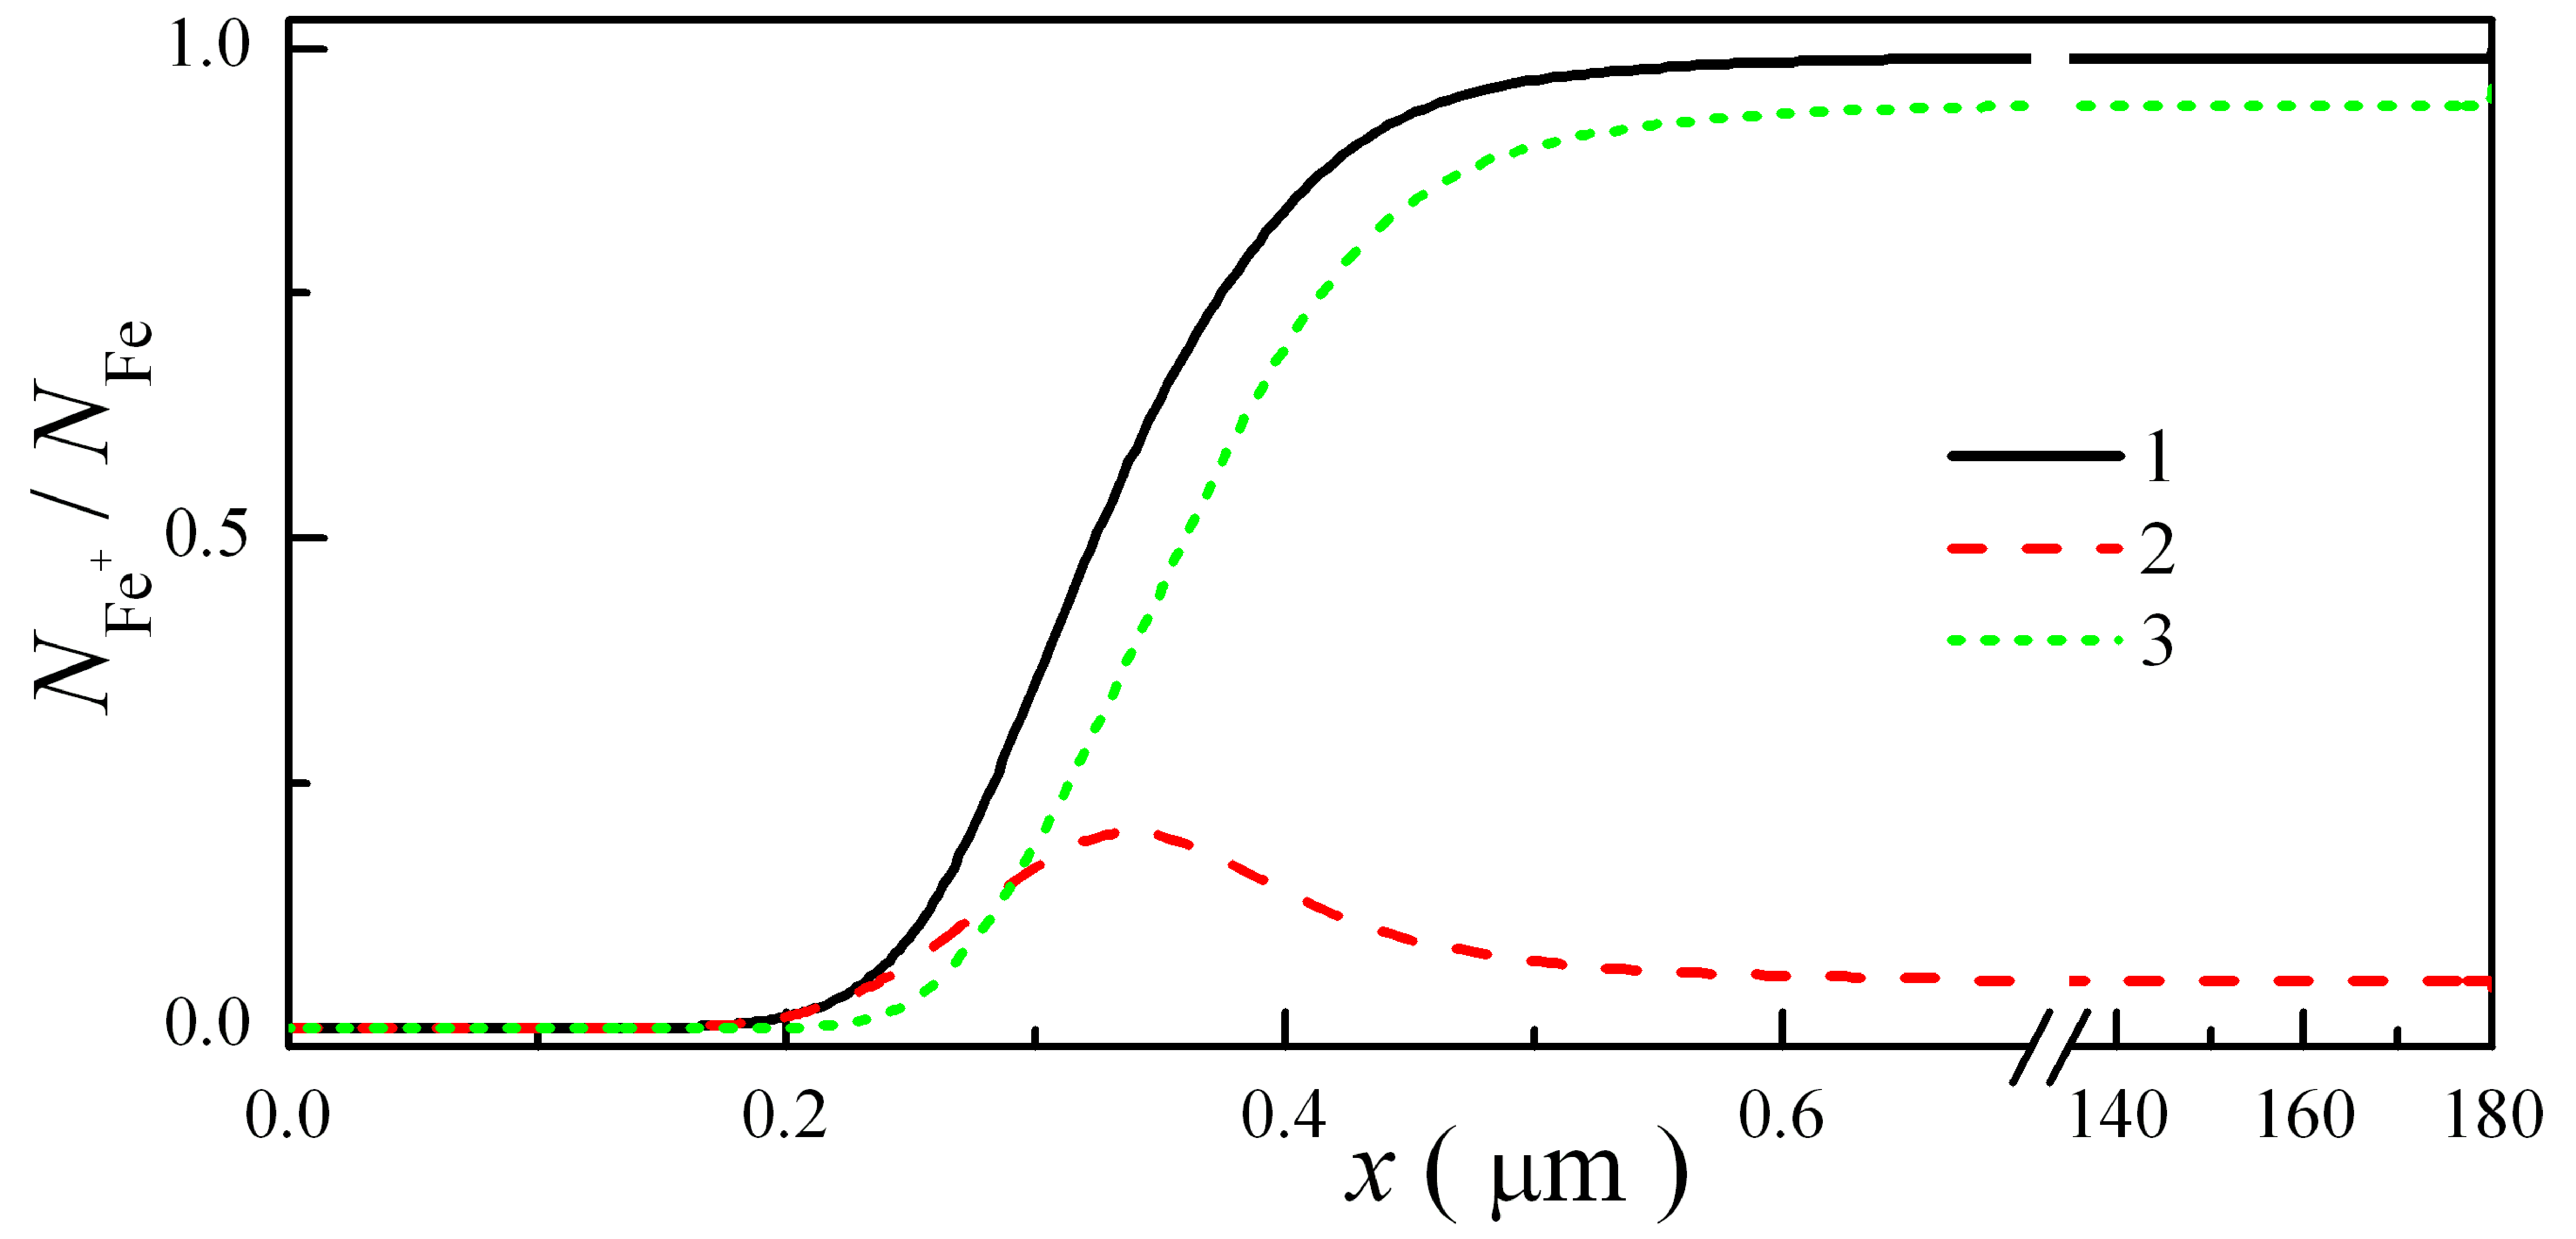
\includegraphics[width=7.5cm]{FigDelFei}
\caption{.
}
\label{FigDelFei}
\end{figure}

\clearpage

\section*{}

\begin{center}
{\bfseries Моделювання фактору неідеальності в $n^+$--$p$--$p^+$--Si структурах}

О.Я. Оліх, O.В. Завгородній

\emph{Київський національний університет імені Тараса Шевченка}

\emph{Україна, 01601, місто Київ, вул. Володимирська, 64/13}

\emph{e-mail: olikh@univ.kiev.ua}

\end{center}

У цій роботі подано результати моделювання величини фактору не\-ідеально\-сті кремнієвих $n^+-p-p^+$ структур.
При цьому вважалося, що основні реком\-бі\-на\-цій\-ні центри у базі структури пов'язані з домішковими атомами заліза.
Для моде\-лю\-вання вольт-амперних характеристик таких структур використовувався Solar Cells Capacitance Simulator (SCAPS).
При цьому додатково враховувалися температурні залежності параметрів як матеріалу, так і дефектів.
При роз\-ра\-хун\-ках вар'ювалися величини рівня легування ($10^{15}\div10^{17}$~см$^{-3}$ атомів бору) та товщини ($150\div240$~$\mu$м) бази,
температура ($290\div340$~K) та концентрації домішки заліза ($10^{10}\div10^{13}$~см$^{-3}$).
Окремо розглядалися випадки, коли всі атоми заліза знаходилися у міжвузольному положенні $\mathrm{Fe}_i$ та
коли переважна частина з них утворювала пари з легуючою домішкою $\mathrm{Fe}_i\mathrm{B}_s$.
Останній випадок відповідає стану рівноваги за відсутності освітлення і при цьому
співвідношення між концентраціями  $\mathrm{Fe}_i$ та $\mathrm{Fe}_i\mathrm{B}_s$ визначалося положенням
рівня Фермі та тем\-пе\-ра\-ту\-рою.
Визначення величини фактору неідеальності ($n$) відбувалося шляхом апроксимації (з використанням
метаеврістичного методу IJAVA) отриманих во\-льт--ам\-пер\-них характеристик.

Показано, що навіть за наявності $\mathrm{Fe}_i\mathrm{B}_s$ основну роль у формуванні величини $n$
відіграють процеси рекомбінації за участю рівнів, пов'язаних з $\mathrm{Fe}_i$.
Залежності $n$ від температури та рівня легування визначаються, насамперед,
заселеністю рівня $\mathrm{Fe}_i$.
У випадку, коли підсилюється відносний внесок процесів власної рекомбінації (високі
температури та рівень легування, низькі концентрації до\-міш\-ки) відбувається зменшення фактору неідеальності.
На величину $n$, окрім концентрації дефектів, впливає також їх просторове розташування відносно $p-n$ переходу.
Зі збільшенням товщини бази структури (у випадку, коли вона перевищує довжину дифузії неосновних носіїв та
переважаючою є рекомбінація Шоклі-Ріда-Хола) відбувається незначне зменшення фактору неідеальності.
По\-ка\-за\-но, що можуть реалізуватися випадки, коли $n$ після розпаду $\mathrm{Fe}_i\mathrm{B}_s$ змен\-шуєть\-ся.
Запропоновано, що зміна фактору неідеальності після розпаду $\mathrm{Fe}_i\mathrm{B}_s$, поряд з абсолютним значенням $n$,  може бути використана
для оцінки концентрації домішок.


\textbf{Ключові слова:}
фактор неідеальності, кремній, $n^+$--$p$--$p^+$ структура, SCAPS, концентрація заліза


\end{document}
